%%%%%%%%%%%%%%%%%%%%%%%%%%%%%%%%%%%%%%%%%%%%%%%%%%%%%%%%%%%%%%%%%%%%%
%% This is a (brief) model paper using the achemso class
%% The document class accepts keyval options, which should include
%% the target journal and optionally the manuscript type. 
%%%%%%%%%%%%%%%%%%%%%%%%%%%%%%%%%%%%%%%%%%%%%%%%%%%%%%%%%%%%%%%%%%%%%

% Langd5 es el template para LANGMUIR
\documentclass[journal=langd5,manuscript=article]{achemso}

%%%%%%%%%%%%%%%%%%%%%%%%%%%%%%%%%%%%%%%%%%%%%%%%%%%%%%%%%%%%%%%%%%%%%
%% Place any additional packages needed here.  Only include packages
%% which are essential, to avoid problems later. Do NOT use any
%% packages which require e-TeX (for example etoolbox): the e-TeX
%% extensions are not currently available on the ACS conversion
%% servers.
%%%%%%%%%%%%%%%%%%%%%%%%%%%%%%%%%%%%%%%%%%%%%%%%%%%%%%%%%%%%%%%%%%%%%
\usepackage[version=3]{mhchem} % Formula subscripts using \ce{}

%%%%%%%%%%%%%%%%%%%%%%%%%%%%%%%%%%%%%%%%%%%%%%%%%%%%%%%%%%%%%%%%%%%%%
%% If issues arise when submitting your manuscript, you may want to
%% un-comment the next line.  This provides information on the
%% version of every file you have used.
%%%%%%%%%%%%%%%%%%%%%%%%%%%%%%%%%%%%%%%%%%%%%%%%%%%%%%%%%%%%%%%%%%%%%
%%\listfiles

%%%%%%%%%%%%%%%%%%%%%%%%%%%%%%%%%%%%%%%%%%%%%%%%%%%%%%%%%%%%%%%%%%%%%
%% Place any additional macros here.  Please use \newcommand* where
%% possible, and avoid layout-changing macros (which are not used
%% when typesetting).
%%%%%%%%%%%%%%%%%%%%%%%%%%%%%%%%%%%%%%%%%%%%%%%%%%%%%%%%%%%%%%%%%%%%%
\newcommand*\mycommand[1]{\texttt{\emph{#1}}}

%%%%%%%%%%%%%%%%%%%%%%%%%%%%%%%%%%%%%%%%%%%%%%%%%%%%%%%%%%%%%%%%%%%%%
%% Meta-data block
%% ---------------
%% Each author should be given as a separate \author command.
%%
%% Corresponding authors should have an e-mail given after the author
%% name as an \email command. Phone and fax numbers can be given
%% using \phone and \fax, respectively; this information is optional.
%%
%% The affiliation of authors is given after the authors; each
%% \affiliation command applies to all preceding authors not already
%% assigned an affiliation.
%%
%% The affiliation takes an option argument for the short name.  This
%% will typically be something like "University of Somewhere".
%%
%% The \altaffiliation macro should be used for new address, etc.
%% On the other hand, \alsoaffiliation is used on a per author basis
%% when authors are associated with multiple institutions.
%%%%%%%%%%%%%%%%%%%%%%%%%%%%%%%%%%%%%%%%%%%%%%%%%%%%%%%%%%%%%%%%%%%%%
\author{Mar\'ia Laura V\'azquez Juiz}
\email{marialvazquez@uvigo.es}
\affiliation[UVIGO Campus Auga]{Facultade de Ciencias, Campus da Auga, University of Vigo}

\author{Diego Soto G\'omez}
\email{disoto@uvigo.es}
\affiliation[UVIGO Campus Auga]{Facultade de Ciencias, Campus da Auga, University of Vigo}

\author{Paula P\'erez Rodr\'iguez}
\affiliation{Instituto Nacional de Investigaciones Agrarias,
Carretera de La Coru\~na km 7,5 Madrid}
\alsoaffiliation{Facultade de Ciencias, Campus da Auga, University of Vigo}

\author{Marcos Paradelo P\'erez}
\affiliation{Department of Agroecology, University of Aarhus}
\alsoaffiliation{Facultad de Ciencias, Campus da Auga, University of Vigo}

\author{Jos\'e Eugenio L\'opez Periago}
\affiliation[UVIGO Campus Auga]{Laboratory of Hydraulics, Faculty of Sciences, Campus da Auga, University of Vigo}
\altaffiliation{Current address:  Edificio polit\'ecnico s/n As Lagoas 32004 Ourense, Spain}
%\email{edelperi@uvigo.es}
\phone{+34 (9)88 387070}
\fax{+34 (9)88 387001}


\title[Resolving particle size of MS by TRPS  in presence of HA ]{Particle size determination with Tunable Resistive Pulse
  Sensing in presence of dissolved natural organic matter\footnote{Resolving particle distribution 
HA-MS mixture suspensions using TRPS}}

%%%%%%%%%%%%%%%%%%%%%%%%%%%%%%%%%%%%%%%%%%%%%%%%%%%%%%%%%%%%%%%%%%%%%
%% Some journals require a list of abbreviations or keywords to be
%% supplied. These should be set up here, and will be printed after
%% the title and author information, if needed.
%%%%%%%%%%%%%%%%%%%%%%%%%%%%%%%%%%%%%%%%%%%%%%%%%%%%%%%%%%%%%%%%%%%%%
\abbreviations{BIC,DLVO,HA,MS,PSD,TRPS}
\keywords{Bayesian Information Criteria, Clustering, Humic Acid, Dejarguin-Landau-Vervey-Oberbeek,Polystyrene-latex Microspheres,Particle Size Distribution,Tunable Resistive Pulse Scanning}

%%%%%%%%%%%%%%%%%%%%%%%%%%%%%%%%%%%%%%%%%%%%%%%%%%%%%%%%%%%%%%%%%%%%%
%% The manuscript does not need to include \maketitle, which is
%% executed automatically.
%%%%%%%%%%%%%%%%%%%%%%%%%%%%%%%%%%%%%%%%%%%%%%%%%%%%%%%%%%%%%%%%%%%%%
\begin{document}

%\tableofcontents
%%%%%%%%%%%%%%%%%%%%%%%%%%%%%%%%%%%%%%%%%%%%%%%%%%%%%%%%%%%%%%%%%%%%%
%% The "tocentry" environment can be used to create an entry for the
%% graphical table of contents. It is given here as some journals
%% require that it is printed as part of the abstract page. It will
%% be automatically moved as appropriate.
%%%%%%%%%%%%%%%%%%%%%%%%%%%%%%%%%%%%%%%%%%%%%%%%%%%%%%%%%%%%%%%%%%%%%
\begin{tocentry}

Some journals require a graphical entry for the Table of Contents.
This should be laid out ``print ready'' so that the sizing of the
text is correct.




\end{tocentry}

%%%%%%%%%%%%%%%%%%%%%%%%%%%%%%%%%%%%%%%%%%%%%%%%%%%%%%%%%%%%%%%%%%%%%
%% The abstract environment will automatically gobble the contents
%% if an abstract is not used by the target journal.
%%%%%%%%%%%%%%%%%%%%%%%%%%%%%%%%%%%%%%%%%%%%%%%%%%%%%%%%%%%%%%%%%%%%%
\begin{abstract}


Dissolved  organic matter (DOM) is ubiquitous the environment and has a great influence on the 
behavior of microorganisms and micro and nanoparticles. Usually, DOM stabilizes particle 
suspensions enhancing their transport. New developments on environmental technical 
applications using this kind of particles require methods of identification and 
quantification. 

%NOM can block the colloid adsorption sites in soil,  aquifers, river beds and packed filters. Can be adsorbed by colloids,  leading the polymer bridging and polymer stabilization. Furthermore,   high concentration of polymer can lead to depletion stabilization of  particles. 

%Coating of colloidal particles by natural polymers  adds complexity on the colloid transport in  porous media.

%Several techniques Light scattering has an intrinsic difficulty to resolve the particle size in polydisperse colloidal suspensions.
Tunable Resistive Pulse Sensing (TRPS) measures the particle size individually. This feature can be used to resolve the components of mixed sizes distributions in the polydisperse aqueous suspensions typically found in natural waters. But little is known about the influence of dissolved polymers on the particle characterization by TRPS.

%TRPS determinations depend on the electrochemical properties of the electrolyte. Presence of natural polymers can affect 

In this work we used TRPS and statistical clustering to distinguish the components of a mixture of particles ($1000~\mathrm{nm}$) and humic acids, HA,  in the range from
$500$ to $2000~\mathrm{nm}$. We differentiated several clusters and studied their behavior with time and different HA concentrations. We found that the presence of HA in the particle suspension increased the size measured by the TRPS, causing an overestimation of the diameter.
\end{abstract}


%%%%%%%%%%%%%%%%%%%%%%%%%%%%%%%%%%%%%%%%%%%%%%%%%%%%%%%%%%%%%%%%%%%%%
%% Start the main part of the manuscript here.
%%%%%%%%%%%%%%%%%%%%%%%%%%%%%%%%%%%%%%%%%%%%%%%%%%%%%%%%%%%%%%%%%%%%%
\section{Introduction}







%Importancia de la distribución de tamaños de los coloides.
Size is the most important factor on the retention of colloidal particles in porous media~\cite{Sirivithayapakorn2003,Sen2006}
Particle size distribution can be dramatically influenced by aggregation and polymer adsorption~\cite{Fang2009}


%=========================================================================
%Aplicaciones 
Understanding  the role of the soil humic polymers in the colloid behavior of natural and engineered particles, in soil and porous media, may contribute to further technical developments based in the control of colloidal processes. The progress in this area will bring important improvements related to water quality, environment, and public health~\cite{Ngo2008}\cite{Farre2011}.

Presence of humic acids (HA) and fulvic acids (FA) has a remarkable influence on the removal of metal contaminants 
\ce{Cr(VI)}  and \ce{As(V)}  by zero-valent Fe nanoparticles~\cite{Mak2011234}.

% Nuevos métodos del conocimiento del suelo
Micro and nanoparticles end up in soils, waters, and  terrestrial environments, through direct application or with wastewater effluents or accidental spillages. Nowadays, we do not know the real effect of many of this substances on the environment or even their amount in soils or waters, so we need new procedures for their identification and quantification. However, particle characterization in natural water samples and aqueous extracts may be cumbersome because of the presence of a huge variety of polymers, colloidal particles and microorganisms~\cite{Ngo2008}
%=========================================================================

%% El problema de determinación de tamaños en suspensiones de tamaños coloidales polidispersos

Dynamic light scattering (DLS)  cannot resolve variation in size as the scattering angle is increased through minima in the intensity form factor. Some efforts have been made to characterize the particle size distributions of colloidal particles with small polydispersities, using a combination of DLS and static light scattering and two-color laser sources to avoid contributions from multiple scattering~\cite{Bryant2003AccurateSuspensions}. However, they report heavy tailed particle size distributions and cannot discriminate different particle size populations.




\subsection{Polymer coating and colloid behavior}

%importancia de la cubierta polimérica y que efectos  tiene sobre el comportamiento de l.os coloides
Polymer coating by DOM affects dramatically the mobility of colloid-size particles in aqueous environments. The ubiquity of dissolved organic matter in these environments makes that polymer-particle interactions have to be considered in all processes in which colloid transport is involved.

For example, the retention of pathogenic microorganisms depends largely on characteristics of the polymer coating~\cite{Morales2011a} . Cross linking can favor the coagulation, bridging and flocculation, enhancing the colloid retention by several orders of magnitude. Conversely,  stabilization by adsorbed polymers can enhance the transport~\cite{Keller2010}.

The conformation of the polymers attached to the particle surfaces is controlled by the cover density, the pH and the ions. These factors determine the polymer coiling. Therefore, the size of suspended colloids vary upon the electrochemical environment~\cite{Morales2011a} .


Study of polymeric coating   on surfaces can be cumbersome.~\citeauthor{doi:10.1021/es981236u}\cite{doi:10.1021/es981236u}
used  \ce{Si/SiO2} wafer strips coated with  polystyrene as support for
adsorption studies of HA laser-beam reflectometry. This procedure is
limited by the technique of coating flat surfaces with a desired compound. Therefore, until now, this method cannot be used to measure the coating in natural colloids or microorganisms.

%Tamaño de los HA (esto puede ir a métodos) de momento no lo  ponemos


%Size of humic acid can be measured by several (electron microscopy, light scattering, size exclusion chromatography).  
%Basic structure and size of soil humic acids from a Dystric Cambisol (WRF) by small-angle X-ray scattering, and small-angle neutron scattering in $50~\mathrm{mM}$ \ce{NaOH\; Na2B3O7} buffer \ce{pH\, 10} was reported ~\cite{Kawahigashi1995}. They reported a core of high electron
%density with a radius of 
%$3.0~\mathrm{nm}$
%surrounded by branches with a radius of gyration between 
%$5.8$ to $7.5~\mathrm{nm}$.


% Métodos disponibles para deteminar el tamaño de los coloides.
%\subsection{State of art on methods to determine  the particle size}

%------------------------------------------------------------------------------------------------------
%esto mejor lo quitamos, complica un poco todo aunque es interesanrte para otros trabajos y para la tesis
%A large amount of work has been done over the double layer interaction of colloids with the same magnitude in their surface charge (same charge or opposite charge). Furthermore, new environmental  applications using micro or nano-scale particles can differ in their surface charge due to the natural DOM. Asymmetric systems show a more complex behavior than the symmetrical ones, and the respective forces have richer features than the symmetrical ones\cite{Ruiz-Cabello2013} .
%------------------------------------------------------------------------------------------------------

\subsection{Tunable resistive pulse sensing}
% En que consiste el TRPS
TRPS method uses the same principle of the Coulter method. It calculates the size of individual particles and determines their  concentration in the sample by counting particle-by-particle within 20 to 3000 nm scale.

%Laura: A qNano (IZON Science) was used in this study, a device that allows measure particle distributions within the nanometer scale. The technique is called TRPS, tunable resistance pulse sensing and when we modify the stretch of the pore at macroscopic level, we modify the size of the nanoscopic pore. 

The measurement procedure consists in applying a voltage across a single pore connecting two cavities. In this way, when a particle passes through the nanopore, there will be a decrease in the applied current. There is a relationship between the voltage and the volume of the particle that crosses so that we can determine the size of the particles by calibration with microspheres of known size. Moreover, the pores are made in a  thermoplastic polyurethane membrane which can be stretched (tunning) to fit the size of nanopore to the best detection of  resistive pulses (blockades) on the passage of the particles~\cite{Weatherall2016}.

%Laura: The set up for the measurements consists of placing the pore membrane in the teeth of the device. The upper and the lower fluid cell have an Ag/AgCl electrode. The pore geometry consists of a conical shape whose smallest aperture lies on the side of the upper fluid cell. The parameters can be adjusted in the device are three: applied voltage, stretch and pressure. The pressure is controlled by a variable pressure manometer (VPM). When the upper fluid cell is full, there is an inherent pressure whose value is 46 Pa which corresponds to the pressure exerted on its container. (Ref.: http://pubs.acs.org/doi/abs/10.1021/acs.analchem.6b01818)

%Ventajas del TRPS 

TRPS has enough resolution to discriminate populations mixed in multimodal samples of polystyrene beads~\cite{Varenne2016MultimodalMethods}.  In adition, this technique does not disturb the geometry of the particle, such as  transmission electron microscopy (TEM) or scanning electron microscopy (SEM), that need the drying of the suspension before measurement.
%inconvenientes

One drawback of the TRPS is the electric conductivity of the buffer used. Electrolyte must meet the requirements of current intensity and voltage for accurate measurements of the blockades. Most of the applications of the TRPS have been developed for biological fluids, and buffers typically used in cellular biology  such as PBS or Tris~\cite{Lane2015}.
The electrolyte constitutes an important limitation in the span of  experimental conditions required in the  earth surface environment, i.e. surface and subsurface waters, with a large range of \ce{pH} and electrolyte composition. Recently, some research is being developed using unbuffered electrolytes at concentrations commonly found in geomedia, 2 mM \ce{KCl} with   pH from  3 to 7 \cite{Mayne2016} .



%
Another limitation is the representativity of the sample. Size is determined in a very small amount of particles, about  $500$ counts in suspensions with $10^9$ particles per liter.



%Por hacer:
%Eugenio .- Efectos de ángulo de trayectoria de las MS sonbre los blockades.
% Produce distribuciones con dos picos, el segundo está asociado a trayectorias con ángulos cerrados.
Under certain experimental conditions, distribution broadening and double peaks can generate significant size measurement uncertainties. Broadening (and hence the uncertainty) can be reduced by working with relatively small pores\cite{Weatherall2016}. This is a potential drawback of the TRPS in aggregation studies: the same pore and stretching  should be used for a large span of aggregate sizes in the same sample.

\subsubsection{Influence of DOM on particle size measurements}

Little in known about the presence of dissolved polymers on the TRPS determinations.  \citeauthor{Pevarnik2013}\cite{Pevarnik2013} reported that hydrogels pass through the pores by electroosmosis and cause a characteristic shape of blockades. Therefore the presence of DOM in natural water samples can alter the  measurements of the particle size. DOM can pass through the macropore in several ways depending on the electrochemical properties of the  suspension and the properties of Dom and the MS surface: DOM can flocculate as a low density  hydro-colloids, can attach to the surface of particles or pass as dissolved together with the  particle thorough the pore. 
 %so we use only the the  full width half-maximum (fwhm), blockade magnitude.

%========================================================================
%Objectives
%========================================================================

In view of above, the TRPS is a promising technique to characterize (nano)-micro particles in water samples from terrestial environments, but the presence of DOM can alter the mesurements. Therefore, the objective is to test the capabilities of TRPS to measure  particle sizes in presence of polymers, in particular   we examine the influence of dissolved natural organic polymers, in particular humic acids, on  particle size determinacion of microspheres using TRPS.

To this aim we examine the influence of several concentrations of HA and contact time between the HA and polystyrene latex MS on the TRPS measurements.



%%%%%%%%%%%%%%%%%%%%%%%%%%%%%%%%%%%%%%%%%%%%%%%%%%%%%%%%%%%%%%%%%%%%%
%% Theory
%%%%%%%%%%%%%%%%%%%%%%%%%%%%%%%%%%%%%%%%%%%%%%%%%%%%%%%%%%%%%%%%%%%%%
%\section{Theory}
%teoría de la formación de recubriemientos poliméricos sobre partículas coloidales
% Gregory, Elimelech


%%%%%%%%%%%%%%%%%%%%%%%%%%%%%%%%%%%%%%%%%%%%%%%%%%%%%%%%%%%%%%%%%%%%%
%% Experimental
%%%%%%%%%%%%%%%%%%%%%%%%%%%%%%%%%%%%%%%%%%%%%%%%%%%%%%%%%%%%%%%%%%%%%
\section{Experimental} % Langmuir
%\section{Materials and methods} %ES&T
\subsection{Particle size measurement}
%Apparatus
The TRPS apparatus is a qNano (iZon Science Europe Ltd., Oxford, UK, serial number 601A-1406-0353), a system that uses the principle of the Coulter method, and the pore used for this experiments was a NP1000 membrane (iZon Science Europe Ltd.). The pore of this membrane can measure particles with a size between 500 and $2000~\mathrm{nm}$ (Figure~\ref{fgr:NPmil}), an optimal interval for measuring the microspheres used in this study.


\begin{figure}
\begin{tabular}{|l|l|}
\hline
A) & B) \\
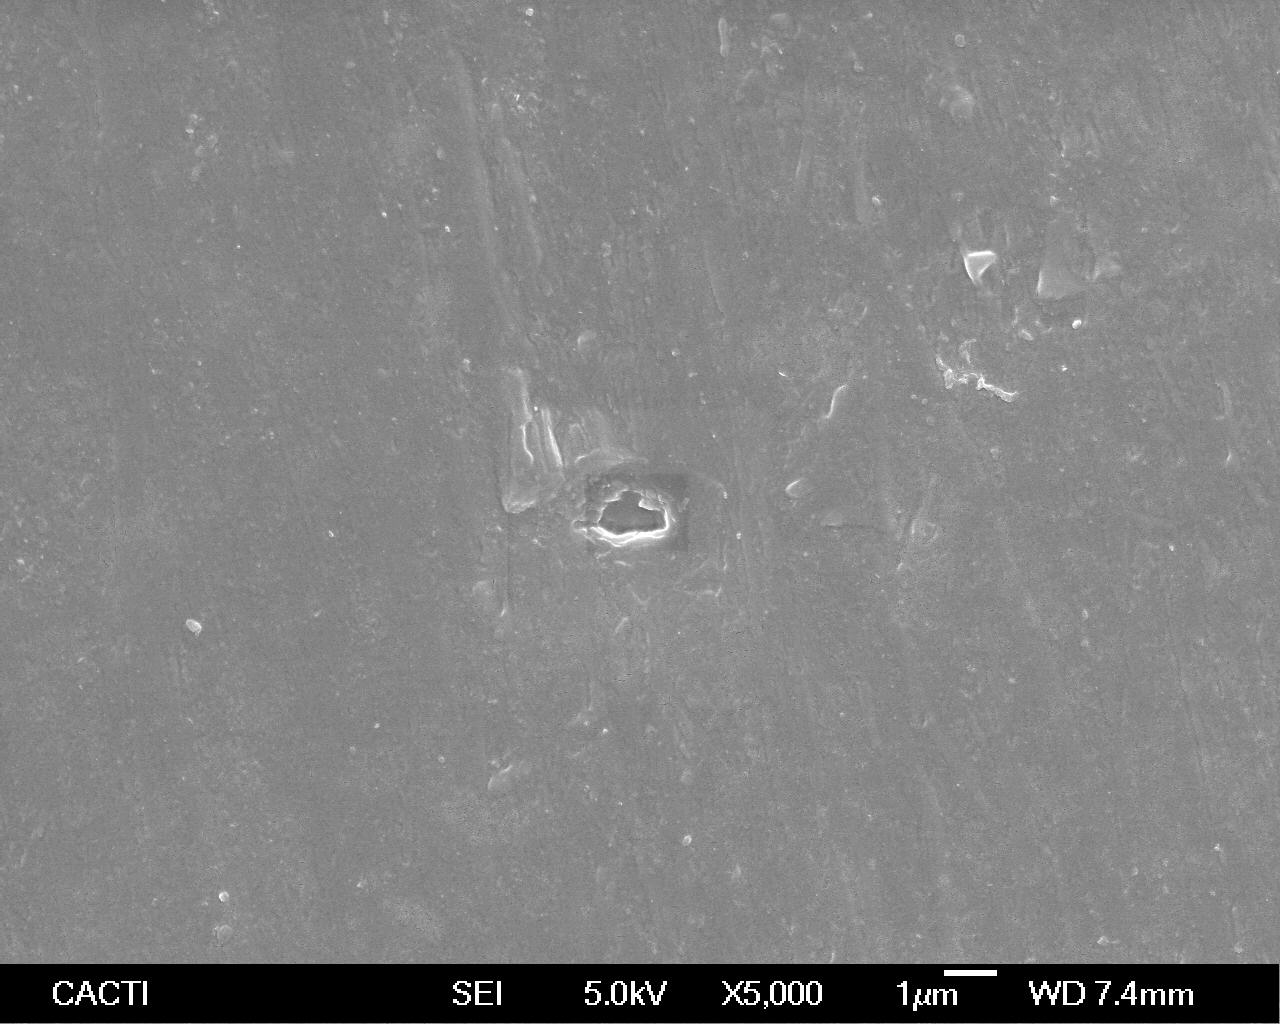
\includegraphics[width=0.5\linewidth]{Figures/NP1000-016.jpg}  &
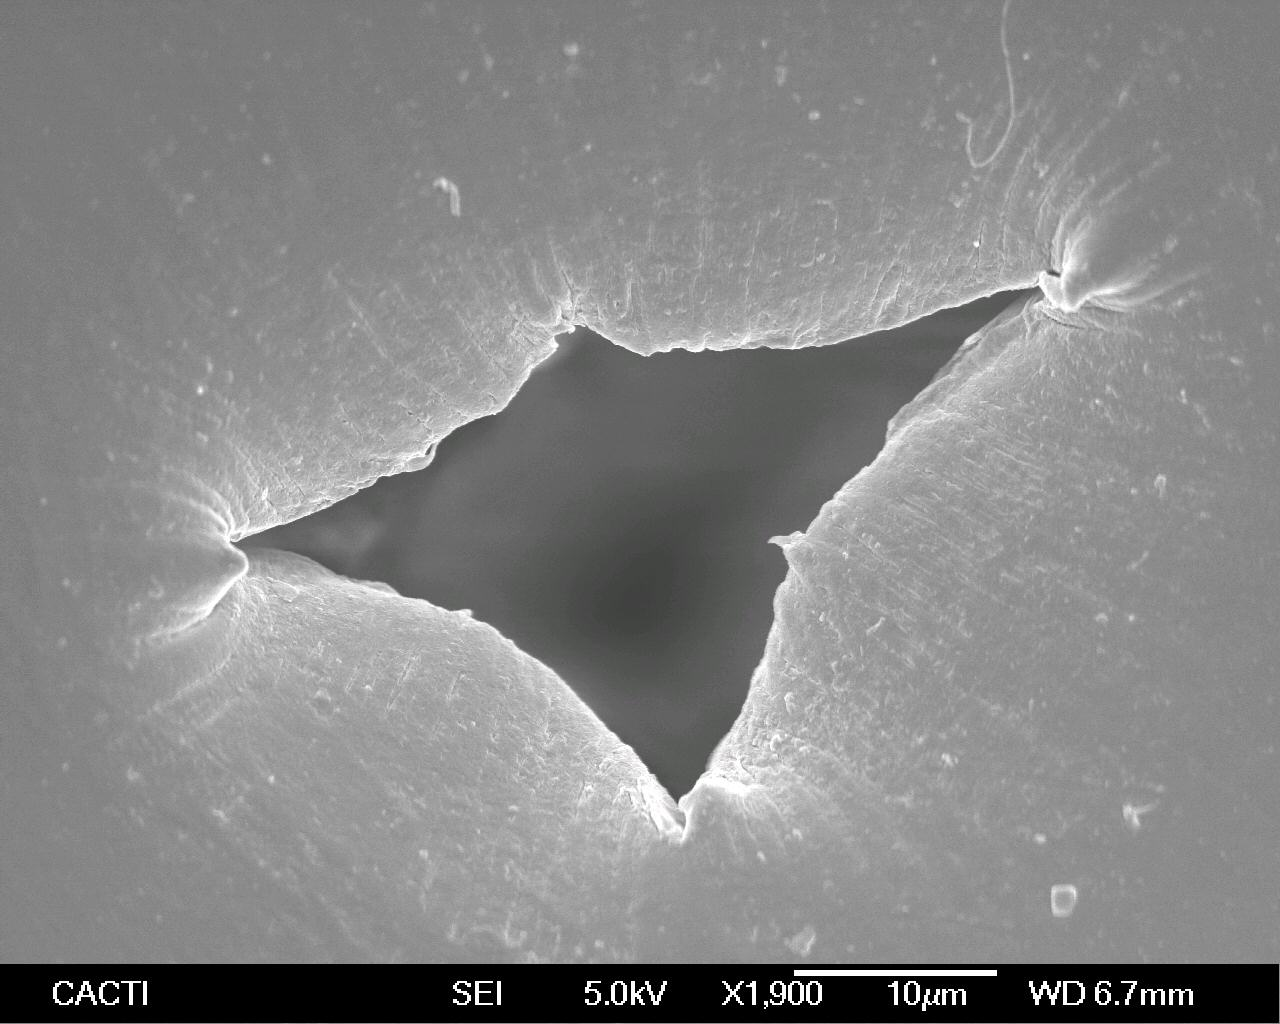
\includegraphics[width=0.5\linewidth]{Figures/NP1000-021.jpg}  \\
\hline
\end{tabular}
\caption{SEM images showing a detail of the pore in the NP1000 membrane. A) x5000: the upper side with  a narrow irregular hole in the center of the image about 1 $\mu m$ in the largest dimension (particle input) , B) x1900: the bottom side is wider hole (particle output). Note that in the image the membrane is not stretched. but it is stretched when installed in the TRPS apparatus, so the shape and size is different during particle measurement.}
\label{fgr:NPmil}
\end{figure}


%Laura: Method employed /measurement protocol/ measurements in the TRPS (protocol): All the buffers were filtered twice after its preparation. The samples were prepared and each one was vortexed for 20 seconds just before injecting in the TRPS apparatus. The vortex that we used was from Phoenix Instrument RS-VA10. For the TRPS measurements, the buffer was put in the lower fluid cell and in the upper fluid cell. The parameters were adjusted to get a current with values between 70 and 150 nA (insert chart with mean values for the current for every measurement). Once the current was stable, the measurement was taken. The buffer was removed from the upper fluid cell and the sample was added. The current must be in the same current value approximately, so the measurement can be taken. The pore we used for all measurements is a NP1000 nanopore (code: A39461) that measures sizes between 500 and 2000 nm. The temperature of the samples was monitored during measurement on the device. The samples were incubated at room temperature (table). 
%The time taken for the measurements was less than a minute for the buffer measurements, 3 minutes approximately for the buffer + HA measurements and the buffer + MS and the buffer + MS + HA measurements lasted a minimum of 30 seconds. The device measurement thresholds are 30 seconds minimum time and 10 minutes the maximum time for the measurement to be optimal, provided that a minimum of >500 blocks is reached for the 30 seconds case. The device parameters were set to 20 units of pressure and a 47.01 mm of stretch. The voltage values depended on the ionic strength of each buffer. To obtain good current values, these voltage values were 0.08 V for the PBS and 0.70 V for NaCl and CaCl2. 



%buffers
All buffers and electrolytes used in the particle size measurements were prepared with ultrapure Milli-Q water (Millipore-Merk)  filtered through a filter membrane of 220 nm pore size. Concentrations of \ce{NaCl} and \ce{CaCl2} were optimized to reach the same operational measurement conditions used with phosphate saline buffer (PBS, \ce{Cl2H3K2Na3O8P2}).

%Laura: Once we had made the buffers, were filtered twice before use to avoid contamination. The qNano apparatus is a very sensitive device, therefore this contamination could give blockades. 

%Colloids
Three types of colloidal suspensions were used in the experiments: microspheres (MS), humic acids (HA), and mixtures of microspheres and humic acids (MS-HA).
Microspheres (Merck-Millipore, Darmstadt Germany, Estapor Microspheres, Ref. F-Y 100, Lot number 953-B1) with a mean diameter of $930 \, \pm 10~\mathrm{nm}$, without surface functional groups. The stock suspension has a polystyrene concentration of $10~\mathrm{g\,L^{-1}}$ (data from the manufacturer).

Humic acids were purchased from Merck-Sigma-Aldrich (humic acid sodium salt technical grade CAS Number 68131-04-4). The molecular weight range of the HA is between  2,000--500,000. HA stock suspensions were prepared by dissolving  $\mathrm{100 \pm 0.5\,mg}$ HA in $100~\mathrm{mL}$ ultrapure water, and vortexed for five seconds using a RS-VA10 vortex stirrer apparatus at maximum speed (Phoenix Instrument, Germany). 

%Pendiente de completar
%Influence of the concentration of HA and incubation time on the size  distribution of MS and electrolyte was evaluated.

\subsubsection{Buffer testing}
Different buffers were tested to select the best measuring conditions, namely, 
152 mM PBS ,
7 mM \ce{CaCl2}, 151.7 mM PBS
and 
14 mM \ce{NaCl} (Table~\ref{tbl:electrolytes}). The suspension of HA, MS and HA-MS in 7 mM \ce{CaCl2} (pH  5.8) were also tested at different times (0.25, 16 and 40 h). All experiments were made in triplicate.

%The MS-HA mixtures were prepared with different concentrations of humic acids: 0, 2, 4, 6, 8 and 10
%$\mathrm{mg\,L^{-1}}$,
%but using always the same concentration of MS of
%$\mathrm{1.0\, mg\,L^{-1}}$,
%latex. 

Mixtures  with different concentrations of humic acids, HA, were prepared to examine their influence on the TRPS blockades. The HA suspensions were prepared from a 
$\mathrm{10\;g\, L^{-1}}$
HA stock suspension. For the different concentrations,  $\mathrm{10\, mg L}$ MS suspension + 
($2, 4, 6, 8, 10~\mathrm{\mu L}$) 
of HA suspension was pippeted into 2-mL capacity eppendorfs vials (Fisherbrand, Fisher Scientific).
%: 2.0 mL MCT Graduated Natural, Cat No. 05-408-138, Qty: 500 PK, Lot 16420813, www.fishersci.com).
The five HA concentrations were evaluated in different times. In amount, we have 8 suspensions: 1 x MS, 2 x HA (2 $\mathrm{\mu L}$ and 6 $\mathrm{\mu L}$) and 3 x MS + HA (2 $\mathrm{\mu L}$, 4 $\mathrm{\mu L}$, 6 $\mathrm{\mu L}$, 8 $\mathrm{\mu L}$ and 10 $\mathrm{\mu L}$). With the suspensions of MS and HA, we can evaluate if coating occurs.

%Samples of microspheres (MS): The microsphere suspensions were a dilution 1:1000 from the stock. This suspension was prepared with 999 uL of buffer and 1 uL of stock that was placed in a 2 mL eppendorf.
%Samples of humic acids (HA): the concentration of this suspension is 1 g/L. The two samples used to measure humic acid calibrations were: a sample prepared with 1000 uL of buffer (7mM CaCl2) with 2 uL and 6 uL of the stock suspension of humic acids. 
%Samples of a microspheres + humic acids mixture (MS + HA): We mixture the 1:1000 dilution suspension of microspheres from the stock plus different volumes of the previous HA suspension. The suspensions that content only humic acids were prepared adding to a eppendorf a 1000 uL buffer plus the corresponding volume of the humic acid stock suspension (2, 4, 6, 8 and 10 uL).


%V búff (uL)	V stock (uL)	V final (uL)	V final (L)	M1 (g/L)	V1 (L)	V2 (L)	M2 (g(L) [M1.V1=M2.V2]	M2 (ppm=mg/L)

%1000	2	1002	0.001002	1	0.000002	0.001002	0.001996008	1.996007984

%1000	4	1004	0.001004	1	0.000004	0.001004	0.003984064	3.984063745

%1000	6	1006	0.001006	1	0.000006	0.001006	0.005964215	5.964214712

%1000	8	1008	0.001008	1	0.000008	0.001008	0.007936508	7.936507937

%1000	10	1010	0.00101	1	0.00001	0.00101	0.00990099	9.900990099



%calculos de la cobertura de HA.
%to know if covering was produced. The MS suspension was a dilution 1:1000 from the stock. 



%Measurement protocol in the TRPS

%Laura: Ajustes TRPS: The current obtained depends on the adjustment of the device parameters, ie. the stretch, the voltage applied and the pore that we use. The pore we used for all measurement is a NP1000 pore (code: A39461). All the buffers have a different ionic strength. The device parameters are set to 20 of pressure and 47.01 of stretch. Depending on the ionic strength of the buffer used, we set a voltage or other. In the case of the NaCl buffer, we had to double the ionic strength. We use two different concentrations (7 and 14 mM) and tested with which of these concentrations we have an optimal current. When using a 7mM NaCl, the current obtained was not in the optimum measurement threshold. With 14 mM NaCl, we had optimal conditions of measurement. The selected voltage for the PBS was 0.08V. At the beginning, pressure was applied for the measure to be carried out, thus more accounts were recorded.



%Suspensions of MS withot HA were prepared in three buffers: \ce{CaCl2},
%PBS and \ce{NaCl}. By mixing 
%$\mathrm{????\, \mu L }$ of the  MS stock suspension
%with 
%$\mathrm{????\, \mu L }$ electrolyte
%in an 1.5 $\mathrm{mL}$ polypropylene vial.

%Laura: Las suspensiones de MS se prepararon haciendo una dilución 1:1000 del stock de las mismas en el búffer correspondiente. Después, se pipetearon 1000 uL de esta suspensión en el eppendorf.

%Laura: Los eppendorfs que se utilizaron son de la marca Fisherbrand (Fisher Scientific): 2.0 mL MCT Graduated Natural 
%Cat No. 05-408-138, Qty: 500 PK, Lot 16420813
%www.fishersci.com


To carry out the measure in the TRPS, the procedure is always the same: $\mathrm{75 \,\mu L}$ of the electrolyte was put in the lower cell and $\mathrm{40 \,\mu L}$  of the suspension (MS, HA or MS-HA) in the upper cell. The parameters were adjusted until get a current with values between 70 and 150 nA, using particle-free electrolyte. Once the current was stable, the samples were injected in the upper cell. The experimental conditions chosen for the three buffers  were identical, with a pore stretch of $47~\mathrm{mm}$. The pressure difference between the two halves of the fluid cell was $66~\mathrm{Pa}$. The above settings were also used by other authors~\cite{Weatherall2016}. The voltages applied were  $0.08~\mathrm{V}$ for PBS, and  $0.7~\mathrm{V}$ for both \ce{NaCl} and \ce{CaCl2}. 
	

% Pressure & Inherent p./ Pa & Inherent p./ cm H2O  & Actual pressure/ Pa & Actual pressure/ cm H2O \\
%\hline
% 20 & 46 & 0.47 & 66 & 0.674347826\\


The settings of iZon-qNano apparatus  for resistive pulse detection are as follows: minimum scan time  time 30 seconds, maximum scan time  10 minutes. Minimum number pulse detections 500. the minimum average detection  rate in 10 min is  $\mathrm{0.83\, s^{-1}}$. 

% Diego:
%Otra forma de decir lo mismo que arriba:
% In our TRPS instrument the measurement times were as follows:
% buffer less than a minute, with less than 4 blockades,
% buffer + HA 3 minutes approximately (about 20 blockades)
% buffer + MS + HA lasted a minimum of 30 seconds, with more than 500 blockades. 


%Experimental plan

%Influence of the concentration of HA and incubation time  on the size  distribution of MS in presence of \ce{CaCl2} electrolyte was evaluated. Five concentrations of HA, namely 2, 4, 6, 8 and  10 $\mathrm{mg\,L^{-1}}$and a control of MS without HA were incubated for 0.25, 16 y 41 h in 7 mM \ce{CaCl2}, pH  5.8. All experiments were made in triplicate.

%Diego. Esto está repe.




%=================== End of the experimental section ==========



\subsection{Particle clustering}

Since clustering is the grouping of similar blockades, some sort of measure could determine whether if blockades represent similar particles or dissimilar. You can find several  clustering methods in the literature:  hierarchical,  partitioning,  density-based,  model-based,  grid-based, and  soft-computing  methods\cite{Rokach2005}.

Partitioning methods (K-means, partition around medoids) are suitable for identifying compact and separated clusters, they require a previous removal of noise and outliers, and the number of clusters that will analyzed. 
Density-based clustering is founded in variations of data density. High density regions surrounded by other with lower densities can be separated by using this method. 
Analysis of particle size apparent populations was done by a model-based clustering. The classification and density estimation of this method is based on finite Gaussian mixture modeling (FGMM). The clustering model used is the expectation-maximization (EM) algorithm. A description  of this algorithm can be read in \citeauthor{Do2008} 
\cite{Do2008}. Briefly, in the FGMM procedure each population of a finite  mixture density is usually associated with a group or cluster. In this work, we assume that all component densities arise from the same parametric distribution family. The model assumes an univariate Gaussian distribution for each component or cluster. In one dimension, there are just two models: all components have equal variance, or different variance among clusters.
With the methods based on finite mixture modeling or density-based clustering, there is no need to specify the number of clusters. The election of the number of clusters affects to the performance of the algorithm. So that, whatever the clustering model, the
determination of the most suitable number of clusters can be done on the basis of the theory of information. In Bayesian
theory, the likelihood of a model is affected by goodness-of-fitting and the number of parameters of the kernel density model, which is proportional to the number of clusters. The criterion used here is BIC (Bayesian Information Criterion).

Details about the clustering procedure and information of the mclust library used for calculations can be read in
~\citeauthor{Fraley2012MclustEstimation}\cite{Fraley2012MclustEstimation}. The mclust library is implemented in the R statistical package~\cite{RCoreTeam2011}.





%%%%%%%%%%%%%%%%%%%%%%%%%%%%%%%%%%%%%%%%%%%%%%%%%%%%%%%%%%%%%%%%%%%%%
%% Results
%%%%%%%%%%%%%%%%%%%%%%%%%%%%%%%%%%%%%%%%%%%%%%%%%%%%%%%%%%%%%%%%%%%%%
\section{Results}
%\section{Results and discussion} %ES&T




%===========================================================
% En esta sección se describen los resultados de probar los
% buffers NaCl y CaCl2
\subsection{Buffers}
%-------------------------------------------------------------
  
  %Masa molecular NaCl 58.44 g/mol
  %Masa molecular CaCl_2  110,98 g/mol
  
  
%LAURA que oncentraciones de MS utilizaste para las pruebas de HA y ? 
%Laura: fue siempre la misma concentración, una dilución 1:1000 con respecto al stock. Para preparar las muestras añadía al eppendorf 1 ml de la suspensión de microsferas y posteriormente añadía el volumen respectivo de suspensión de ácidos humicos (2, 4, 6, 8 y 10 uL)


Optimal conditions of baseline current magnitude, stability and blockade readings were obtained with the electrolytes shown in Table~\ref{tbl:electrolytes}. 

%!!!!!!!!!!!!!!!!!!!!!!!!!!!!!!!!!!!!!!!!!!!!!
%  LAURA:     

%Búffer / Mol. Mass (g/mol)	[  ]/ mM	Ionic strength/ mM	pH medido
%PBS (Cl2H3K2Na3O8P2)	411.038452	151.7	171.7	7.55
%NaCl	58.44277	14	14	6.21
%CaCl2	110.984	7	21	5.8

%PBS: https://pubchem.ncbi.nlm.nih.gov/compound/24978514#section=Top


\begin{table}
\caption{Characteristics of the electrolytes used in the TRPS
measurements and optimal voltage in the measuring cell using an iZon NP1000 micropore.}
\label{tbl:electrolytes}
  \begin{tabular}{lrrrr}
Electrolyte & Conc. & \ce{pH}  & $I$ & voltage\\
\hline
PBS &	152 & 7.55	&	172 & 80 \\
\ce{NaCl} &	14	& 	6.21 &	14 & 700\\
\ce{CaCl2} &	7	& 5.8 &	21 & 700\\
\hline
\multicolumn{4}{p{0.42\linewidth}}{
Conc., concentration ($\mathrm{mmol\,L^{-1}}$); 
$I$, ionic strength  ($\mathrm{mmol\,L^{-1}}$); 
Voltage, ($\mathrm{mV}$).
}
\end{tabular}
\end{table}
%!!!!!!!!!!!!!!!!!!!!!!!!!!!!!!!!!!!!!!!!!!!!!


 
 % Testing the background blockades using buffers and HA
The  \ce{CaCl2} ($\mathrm{7\, mmol\,L^{-1}}$, $\mathrm{pH}\,5.8$) electrolyte without
HA or MS gave about six blockades after $\mathrm{600\,s}$
(Table~\ref{tbl:baseline_blockades}). These measurements are caused by some contamination and are quite normal. In the (Table~\ref{tbl:baseline_blockades}) we
also showed the blockade rate, that is the sum of the magnitudes of all blockades
(nA) divided by the time of measure (s). The rate of blockades, using the highest
concentration of HA ($10~\mathrm{mg\,L^{-1}}$) in \ce{CaCl2} and 40 h of incubation
time, was $0.042\,\pm0.059~\mathrm{nA\,s^{-1}}$.
On the other hand, the rate using  MS in \ce{CaCl2} was 240 times higher than only with HA. Therefore,  blockades of dissolved HA  can be neglected, and all the blockades in  HA-MS mixtures can be assigned to the MS.

 

\begin{table}
\caption{Comparison of the average blockade rates ($\mathrm{nA\,s^{-1}}$), and accumulated nA in 10 minutes between MS
and HA ($10~\mathrm{mg\,L^{-1}}$)
in \ce{CaCl2} $\mathrm{7\, mmol\,L^{-1}}$. The control is electrolyte without colloid or Ha. The tests were made in triplicate.
}
\label{tbl:baseline_blockades}
\begin{tabular}{
l r@{$\pm$}l 
r
}
Test & \multicolumn{2}{c}{blockade rate} &AcnA10\\
\hline
MS & 10.1 & 2.66 & 6057 \\
HA  & 0.042  & 0.059 & 25\\
\ce{CaCl2} only & 0.008 & 0.007 & 5\\
\hline
\multicolumn{4}{p{0.4\linewidth}}{
Blockade rate in $\mathrm{nA \,s^{-1}}$;
AcnA10, accumulated  nA in 10 min} 
\end{tabular}
\end{table}



%Estrutura de los datos de bloqueo y duración
\subsection{Influence of the buffer on the size of blockades}

A comparison of blockade magnitude and duration for the PBS, used as reference  buffer, and \ce{NaCl} and \ce{CaCl2} electrolytes is shown in Figure~\ref{fgr:pairs_buffers}.
The scattering patterns observed using  \ce{NaCl}  and \ce{CaCl2} are similar, while the ones obtained with PBS showed a largest dispersion in blockade duration.
%%=============================================================
 \begin{figure}
  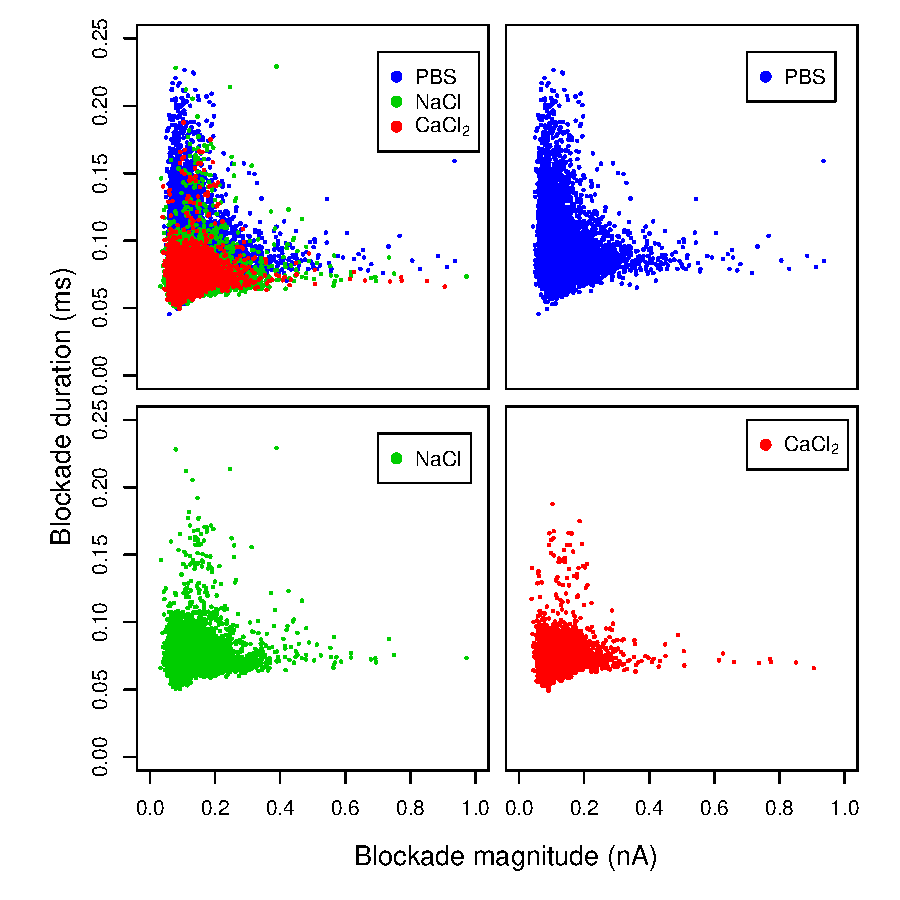
\includegraphics[width=\linewidth]{Figures/Raw_Pairs_buffers_MS_T0_Fwhm.pdf}
%  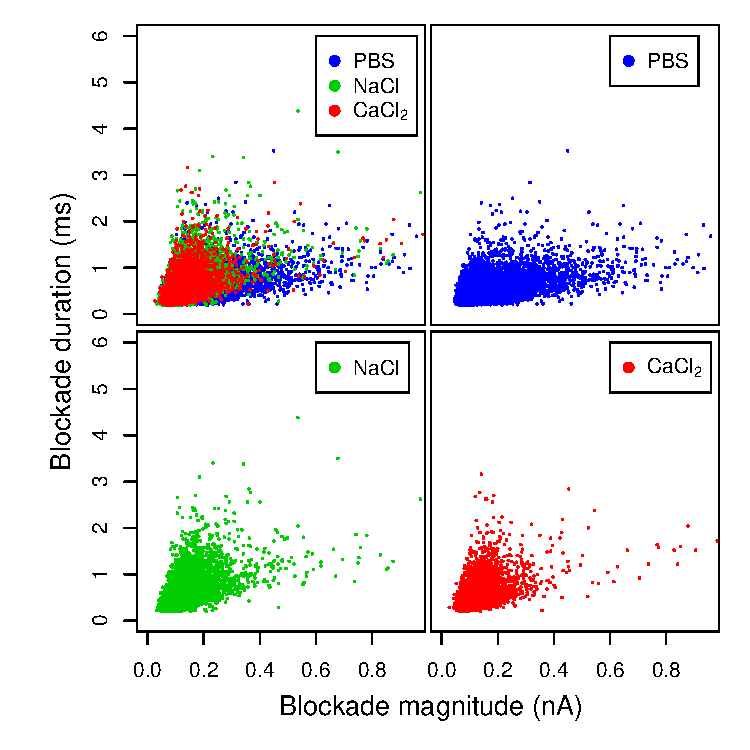
\includegraphics[width=\linewidth]{Figures/Pairs_buffers_MS.pdf}
  \caption{Scatter-plot comparing  blockade magnitude and
  blockade duration of  the polystyrene MS for three
  electrolytes without humic acids. The core of the point cloud is similar in the three electrolytes. PBS  presents the largest dispersion in the blockade magnitude. The number of blockades in clouds is: for PBS 5610; for \ce{NaCl} 7100 and for \ce{CaCl2} 8067. All measurements were made in triplicate using the NP1000 pore, $0.5~\mathrm{V}$ of voltage and a pressure of $2~\mathrm{kPa}$.} 
  \label{fgr:pairs_buffers}
\end{figure}
%% ========================================================






The  distribution of cloud points of blockades magnitude versus duration in all the experimental design can be examined in Figure~\ref{fgr:blockades}. In this figure, we used the full width half-maximum (fwhm) in order to get a reduction of the noise of the baseline. Incubation time and [HA]  increase the dispersion of the cloud of points toward higher blockade magnitude values. It is important to note the decrease of the blockade rate with incubation time, which was more marked in absence of HA.
%Eugenio: quedei !

 \begin{figure}
  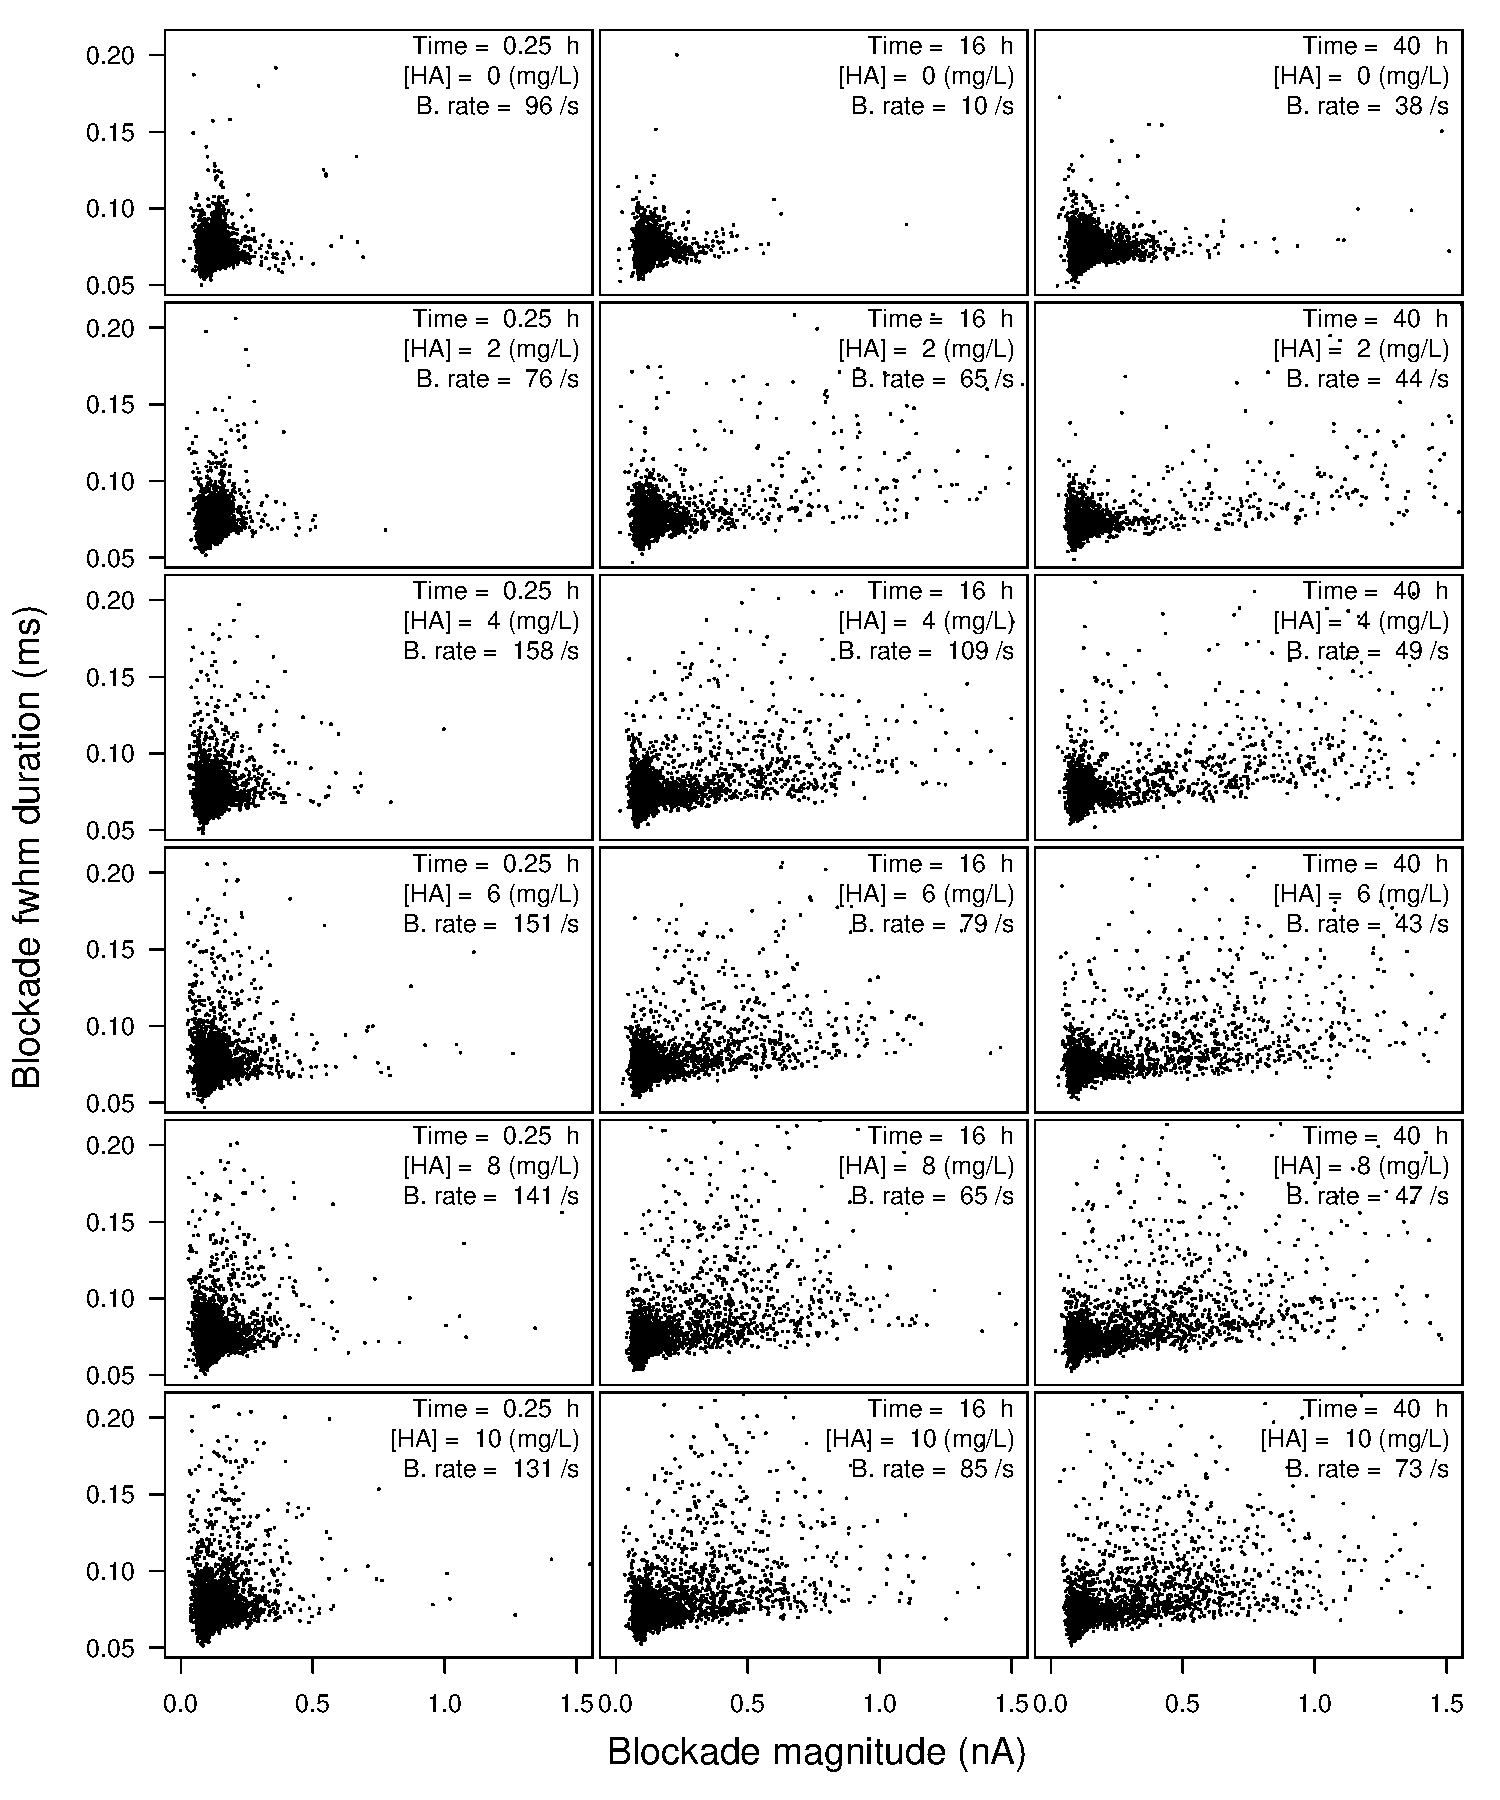
\includegraphics[width=\linewidth]{Figures/Scattering_MS_HA_D2_detail.pdf}
  \caption{Influence of concentration of HA and incubation time on the blockade magnitude of MS in 7 mM~\ce{CaCl2} using a NP1000 (1000 nm pore size). The insets indicate the incubation time, the concentration of humic acids and the blockade rate (B. rate) per second. Incubation time and [HA] increased the span of blockade magnitudes and decreased the blockade full  width half-maximum (fwhm) rate, i.e., the duration of the blockade at maximum height.}
\label{fgr:blockades}
\end{figure}



Analysis of the waveforms of blockades in presence of HA shows anomalous resistive pulses
(Figure~\ref{fgr:block_sorting_HA6_T16}).
Anomalous  waveforms were less than  $4\%$
(Figure~\ref{fgr:block_sorting_HA6_T16}b).
but large waveforms were about $11\%$   
(Figure~\ref{fgr:block_sorting_HA6_T16}c).

%====================== Blockade sorting =====================================
 \begin{figure}
  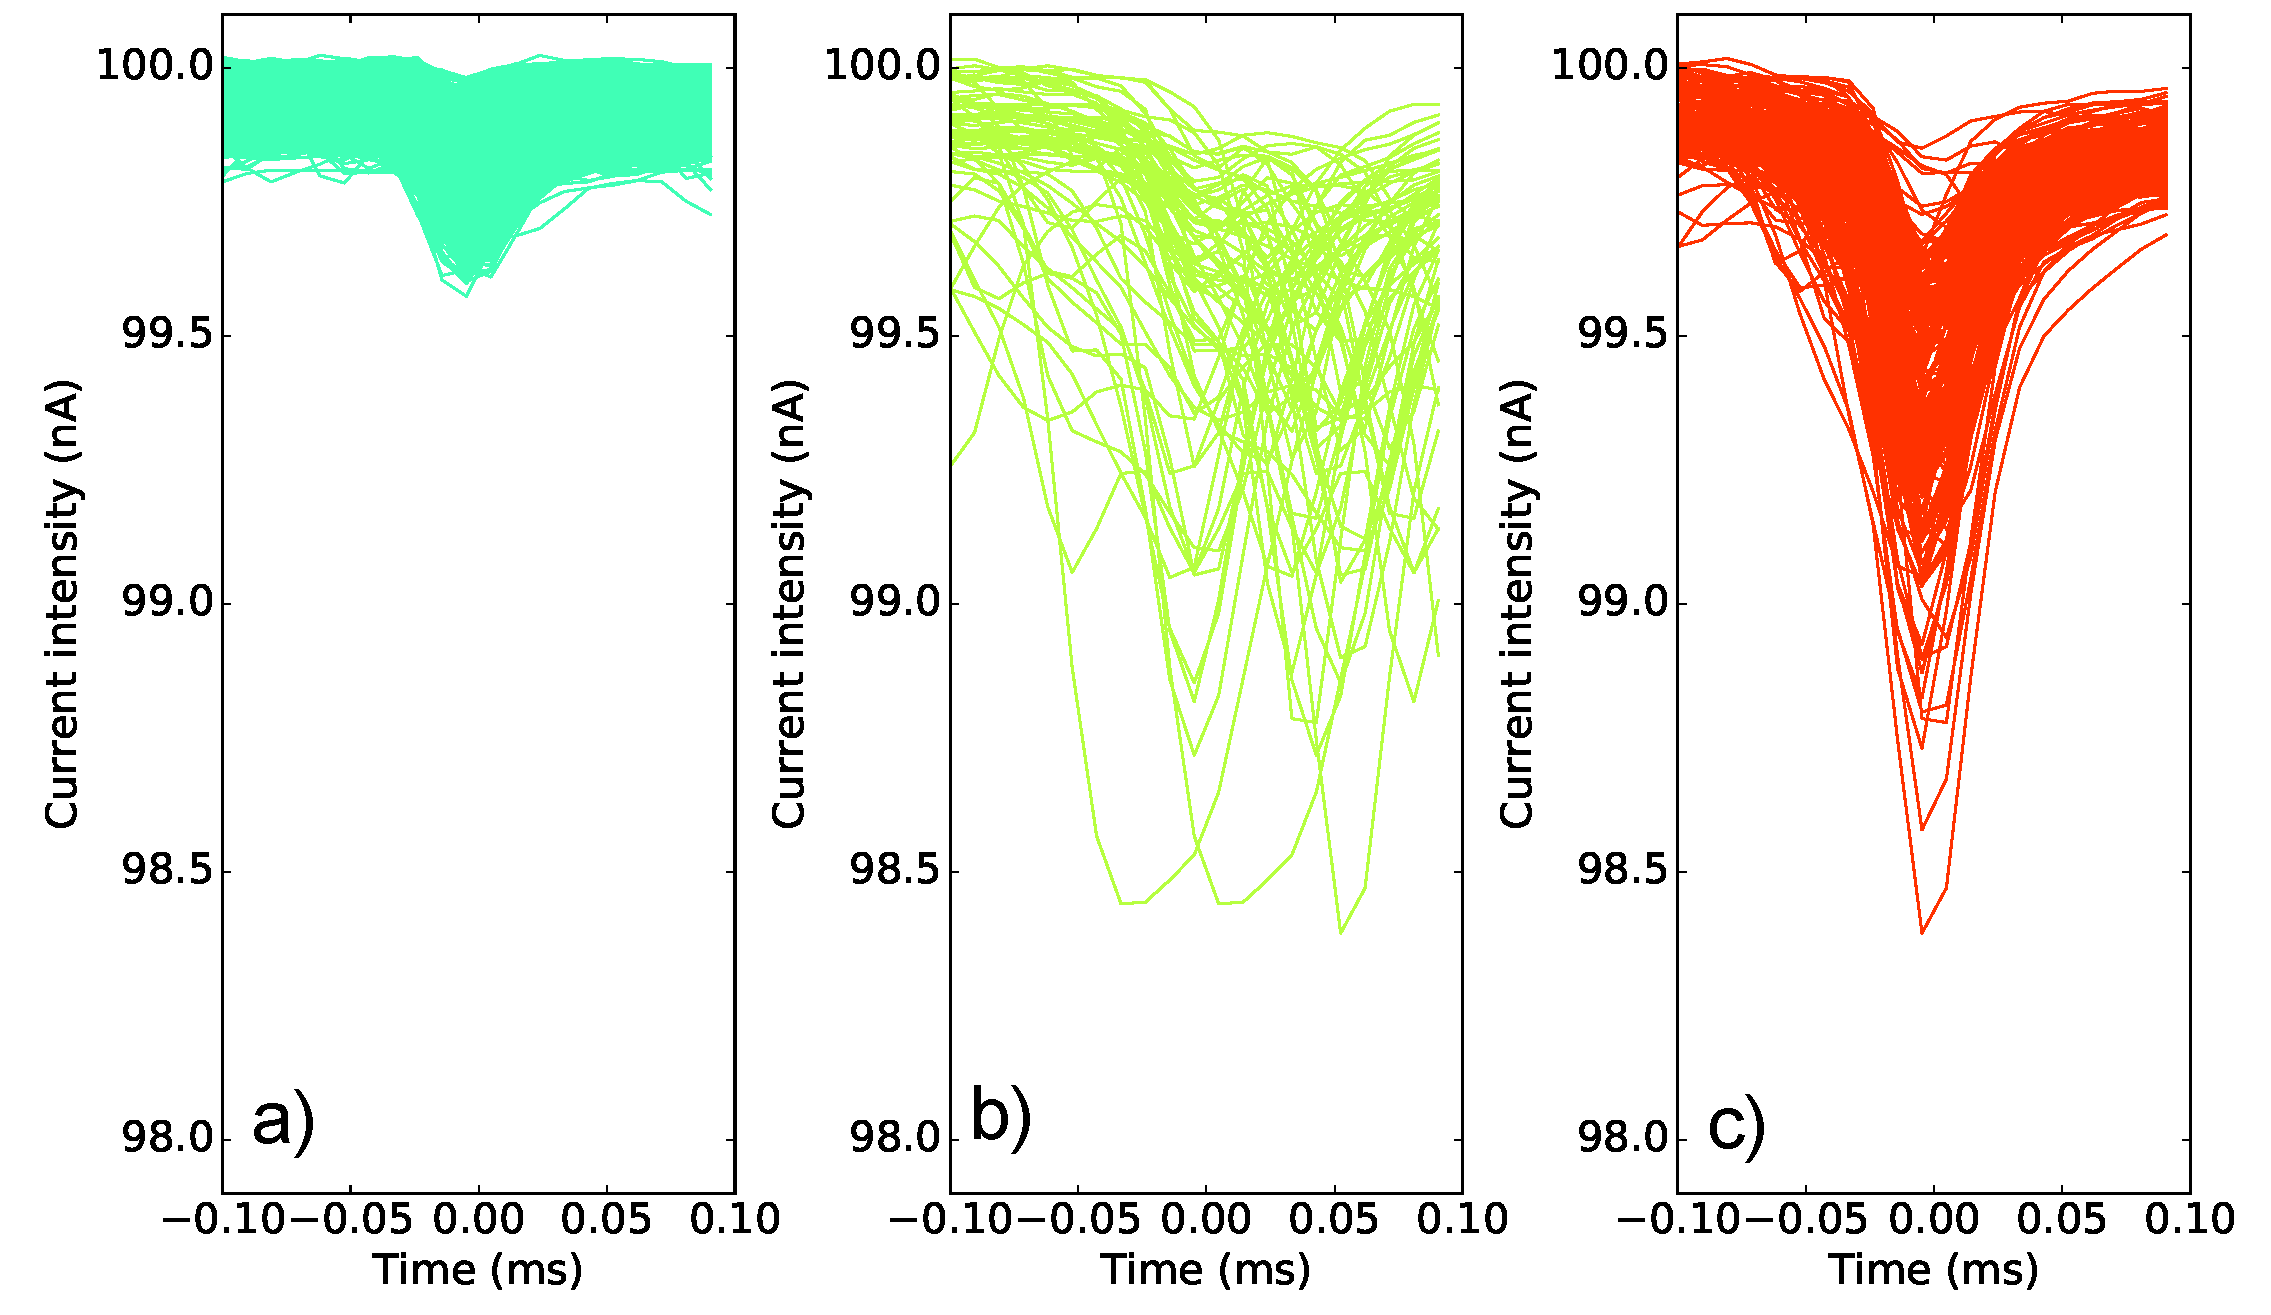
\includegraphics[width=\linewidth]{Figures/Block_sorting_HA6_T16.pdf}
  \caption{Waveforms corresponding to resistive pulses  after a measurement of a mixture of MS and $\mathrm{6\, mg\, L^{-1}}$ HA incubated for 16 h. Waveforms were detected with using a threshold the 5 times the median absolute deviation. The waveforms a aligned in such way that peaks coincide at t =0 in a time frame  of 200 ms duration. The Waveforms were sorted using principal component analysis projection  and the finite gaussian mixture model based on expectation-maximization algorithm. Three main shapes were identified, namely,  a) regular waveforms corresponding to 1606 blockades, b) anomalous waveforms with double peaks and asymmetric tails (70 blockades) and c) large waveforms 209). Baseline current was 100 nA.}
\label{fgr:block_sorting_HA6_T16}
\end{figure}
%==================================================================================


Blockade magnitude and duration were also analyzed  by 2D clustering methods using the normalized transformation \cite{Weatherall2016,VogelQuantitativeSizing2011}. The  standard sizing technique consists in calculating the cube roots of TRPS pulse magnitude, normalized by their mean value. Pulse duration was also normalized  dividing by the mean values.

Table~\ref{tbl:clusteringbuffers} shows that the number of blockades was similar for the three buffers.

Examining the 2D FGMM  clustering  for blockades, using 7 mM \ce{CaCl2}, the algorithm shows an optimal fit using 6 BIC. Moreover, that results in a over-fitting.   

\begin{table}
\caption{2D  clustering results of blockade magnitude and  duration for the three buffers, using the gaussian finite mixture model, and fitted by the EM algorithm}
\label{tbl:clusteringbuffers}
\begin{tabular}{rrrrrrr}
& \multicolumn{2}{c}{\ce{CaCl2}} &
  \multicolumn{2}{c}{\ce{NaCl}} &
  \multicolumn{2}{c}{PBS} \\
\hline
\# & Nb. & MP &
    Nb. & MP &
    Nb. & MP \\ 
\hline
1 & 13 &  0.004  & 1068 &   0.328 &  447 &    0.119 \\
2 & 587 & 0.137  & 988 &    0.283&   342 &    0.107 \\
3 & 1340 & 0.357 & 739 &    0.237&   787 &    0.206 \\
4 & 1332 & 0.343 & 231 &    0.077&   713 &    0.215 \\
5 & 331 & 0.106  & 174 &    0.062 &  80 &     0.019 \\
6 & 76 &  0.022  & 8 &      0.003 &  1059 &   0.291\\
7 & 72 &  0.032  & 18 &     0.009 &  54 &     0.017 \\
8 &    &         & 2 &      0.001 &  104 &    0.024 \\
\hline
Sum &3751 &&  3288  && 3586 &  \\   
\hline
\multicolumn{7}{p{0.5\linewidth}}{Nb., number  of blockades in the cluster ;MP, mixing probabilities.}\\
\end{tabular}
\end{table}





\subsection{HA-MS interaction}

The HA-MS case is a clear example of asymmetrically charged colloids and surfaces. The charged-neutral interaction can be calculated within the Debye-Huckel (D-H) model. Theoretical calculations of colloid-sphere interactions using the Dejaguin-Landau-Vervey-Oberbeek, DLVO, approach (see Table~\ref{tbl:dvlo_interaction}), showed that there is not a repulsive barrier (Figure~\ref{fgr:SEM_50000X}A). The attraction potential at 1 nm separation, in absolute value,  is $12\;k_B\,T$ ($\;k_B\,$is the Boltzmann constant, and $T$ is the temperature). That results in a very weak long-range interaction.
%The potential is  much less than the reference values for colloid adsorption  of
%$20\;k_B\,T$\cite{Adamczyk1999}. 
%quedei

%%==============================================================
\begin{table}
\caption{Double layer sphere-sphere interaction  of HA and MS using the standard DLVO calculations, assuming constant potential.}
\label{tbl:dvlo_interaction}
\begin{tabular}{lrl}
Variable & Magnitude & Units\\
\hline
Temperature & 298 & K\\
Boltzmann constant ($K_\mathrm{B}$) & $1.3806\,10^{-23}$ & $\mathrm{J\, K^{-1}}$\\
Hamaker constant & $7.9\,10^{-21}$ & J\cite{Fronczak2017}\\
MS  diameter & $9.5\, 10^{-7}$ & m\\
HA  diameter & $9.0\, 10^{-9}$ & m\\
HA surface potential & $-40$ & mV\cite{Rodrigues2009}\\
MS surface potential & $-3$ & mV\cite{Kotera1970}\\
Ionic strength & $7$ & mM \\
Regulation parameter of the HA & 0.5 \\
Debye-Huckel constant & $3.9\,10^8$ & $\mathrm{m^{-1}}$\\
%Repulsion barrier & $0.15$ & $\mathrm{K_B\,T}$\\
\hline
\end{tabular}
\end{table}
%===============================================================

In addition to theoretical calculations, scanning electron microscopy (SEM), did not show any influence of the HA in the morphology of the latex microspheres (Figure~\ref{fgr:SEM_50000X}B and C). This means that the adsorption of HA on MS in 7 mM \ce{CaCl2} was negligible, and confirms the small energy interaction predicted by the D-H model. However, a repulsive barrier can exist because of the asymmetric interaction of charged HA and uncharged MS. This point will be discussed later.

%%===================================================================== 
 \begin{figure}
 \begin{tabular}{|l|l|}
 \hline
  A) & B)\\
  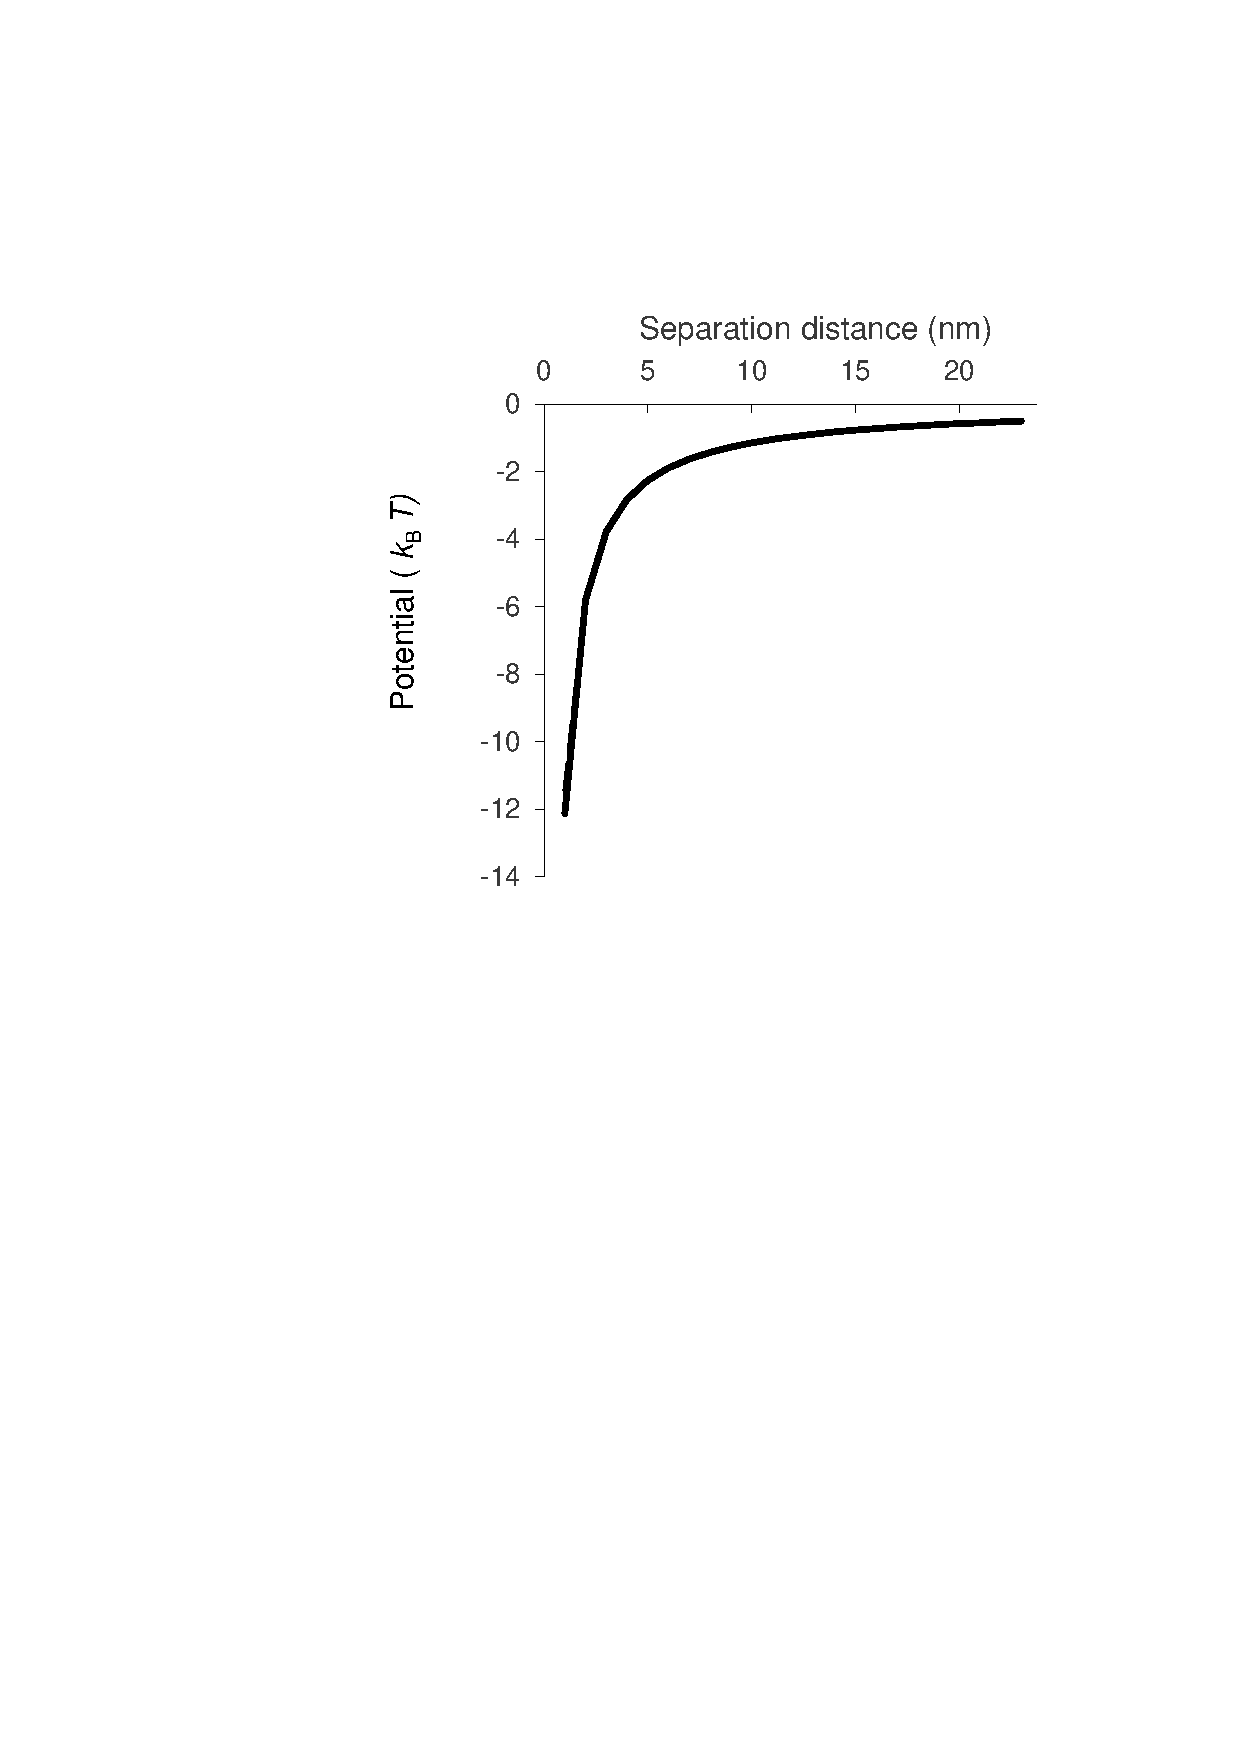
\includegraphics[width=0.49\linewidth]
  {Figures/HA_MS_Laura_DLVO.pdf} & 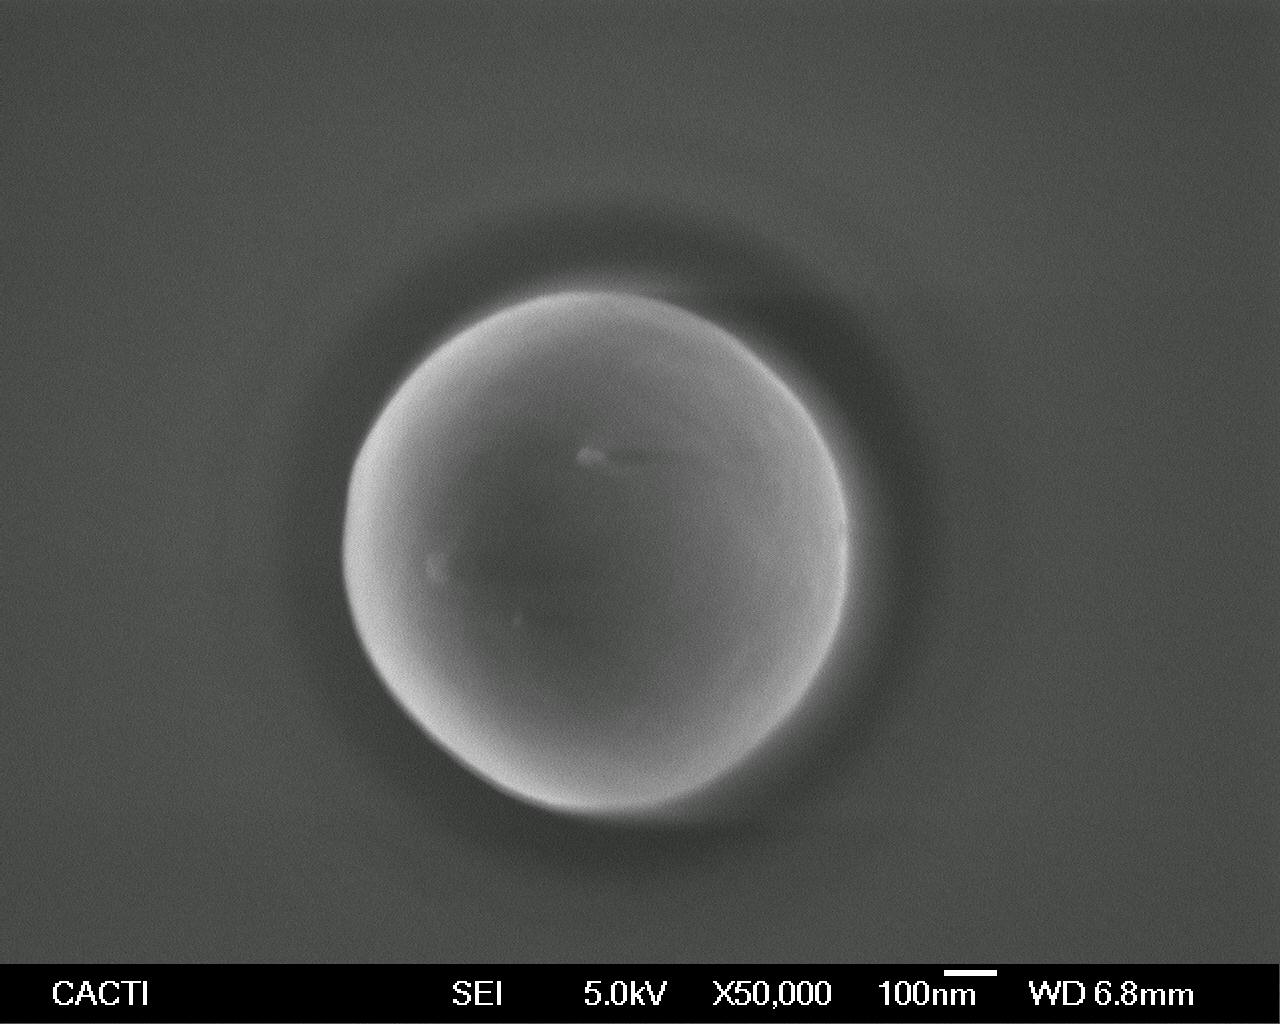
\includegraphics[width=0.49\linewidth]{Figures/5-063.jpg}\\
 \hline 
  C) & D)\\
  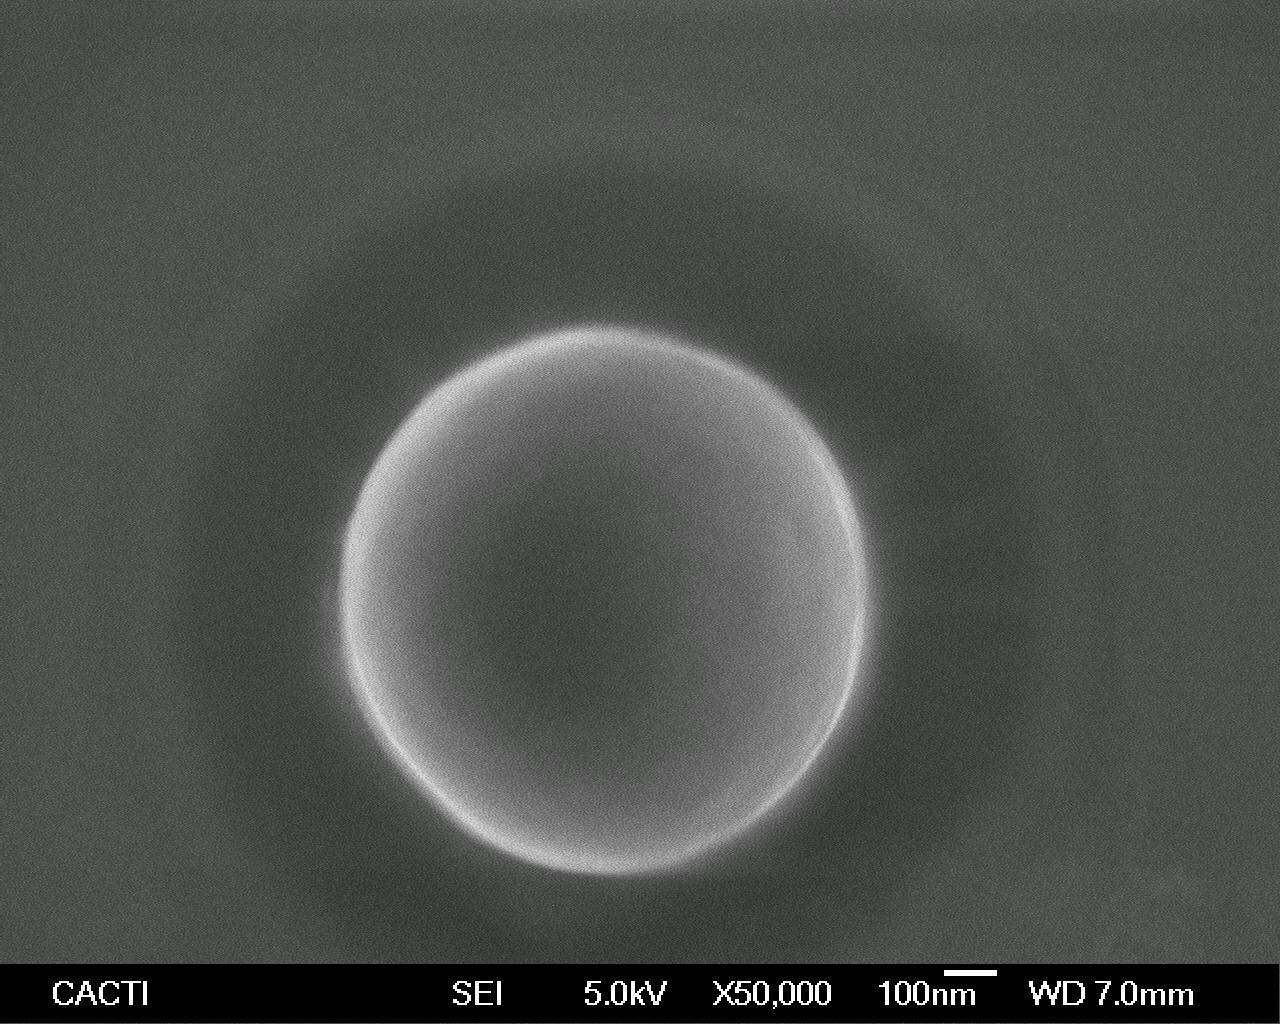
\includegraphics[width=0.49\linewidth]
  {Figures/4-052.jpg} & 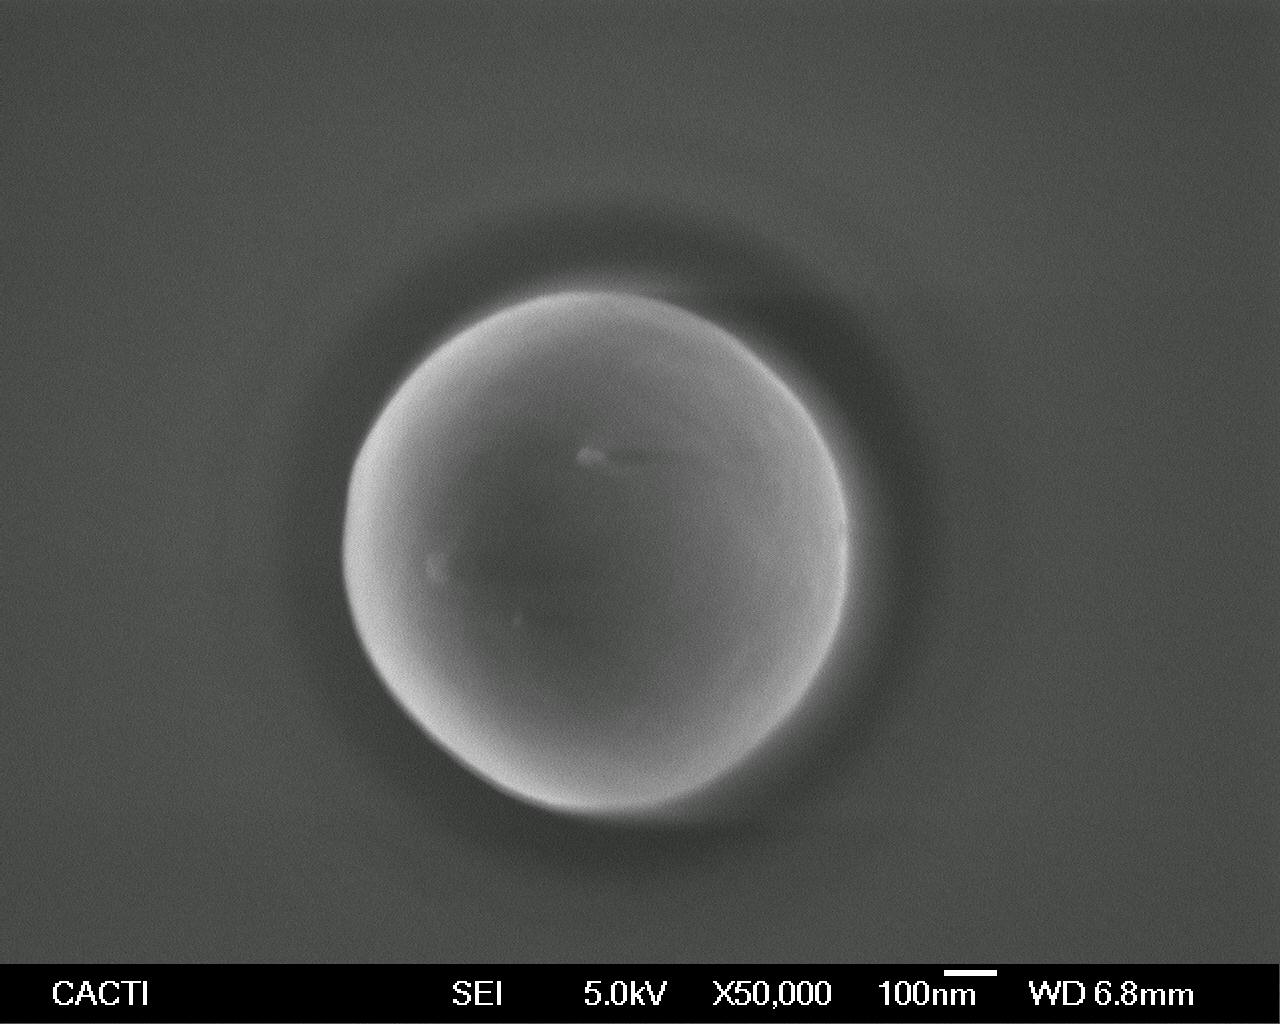
\includegraphics[width=0.49\linewidth]{Figures/5-063.jpg}\\
 \hline
  \end{tabular}
  \caption{A) Calculated DLVO interaction energy as a function of separation distance between the humic acid and the latex particle in \ce{CaCl2} 7 mM; and B, C) SEM images showing two microspheres (x50000): B) without humic acids in 7 mM \ce{CaCl2}, and C)  with 10 mg/L of humic acids after 10 h of incubation. Presence of HA can not be noticeable from the SEM images.} 
% * <diego.cerreda@gmail.com> 2017-06-19T15:02:48.446Z:
% 
% > \caption{A) Calculated DLVO interaction energy as a function of separation distance between the humic acid and the latex particle in \ce{CaCl2} 7 mM; and B, C) SEM images showing two microspheres (x50000): B) without humic acids in 7 mM \ce{CaCl2}, and C)  with 10 mg/L of humic acids after 10 h of incubation. Presence of HA can not be noticeable from the SEM images.} 
% >   \label{fgr:SEM_50000X}
% > \end{figure}
% 
% Borrar imagen D. Está repe.
% 
% ^.
  \label{fgr:SEM_50000X}
\end{figure}
%% =========================================================================




%Resultado: Flocculation excesiva por elevada fuerza iónica
High ionic concentrations can flocculate colloids in a few minutes. High flocculation rate implies that the aggregate size distributions shift towards bigger sizes, much larger than the range of the measuring pore used in the TRPS. In addition, the presence of large flocs in the conductivity cell of the TRPS precludes the small particles enter into the pore membrane. That results in low particle counts that are not representative.

After several trials we found the optimal conditions for the particle size measurements:  \ce{[CaCl2] \; 7\, mmol\, L^{-1}} and \ce{pH \; 6.4 \pm0.2}.
%poner  fotografías de los flocs 
% revisar este dato de pH porque el pH-metro no calibraba muy bien







\subsection{Influence of HA on particle size}

%Evolución global de los tamaños
TRPS measurements indicated an increase of the size of the MS after the addition of HA (Figure~\ref{fgr:meansize}). The contact time also had a notable influence on that increased size. At short times, $< 1~\mathrm{h}$, presence of HA was negligible, but large times, $16 - 40~\mathrm{h}$, produced a large increase in size. This seems to contradict the SEM images and the D-H calculations.

%%============================================================= 
 \begin{figure}
  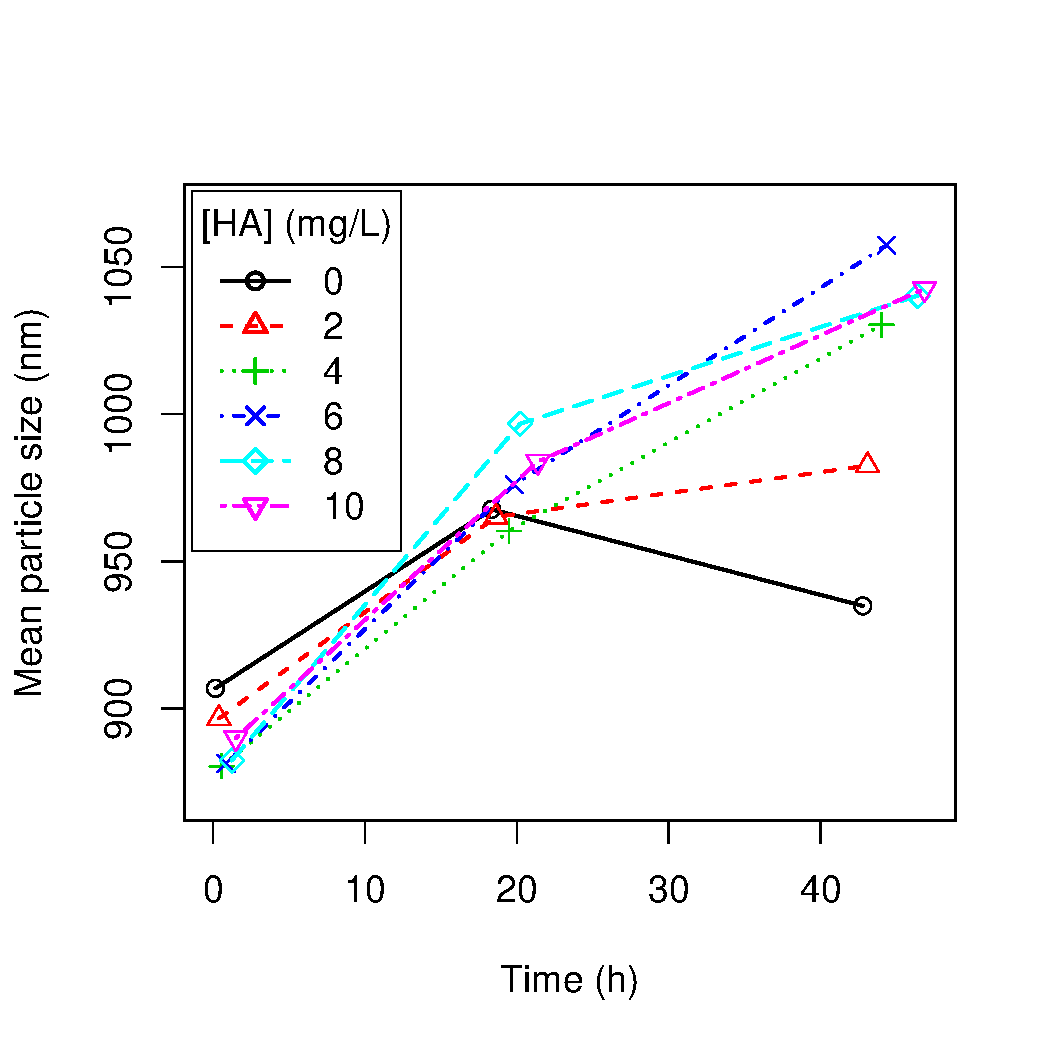
\includegraphics[width=\linewidth]{Figures/mean_particle_size.pdf}
  \caption{Time course of the evolution of the particle size, calculated by the  ratio moment 4 divided by the moment 3, for different concentrations of humic acids.} 
  \label{fgr:meansize}
\end{figure}
%% ============================================================

% En esta parte solamente describimos los resultados, no aventuramos ninguna 
%  ya sabemos que los HA en CaCl2 NO producen Blockades (apenas) :-)!!!!

%Gaussian finite mixture model fitted by EM algorithm   

The optimal  kernel density function was, in general, fitted with a mixture of three gaussian components with different variances. In one case, $0.25~\mathrm{h}$ and $\mathrm{[HA]\, = 6\, mg\,L^{-1}}$, the optimal presented four components. The density histograms and the best fitting  kernel density plots, (Figure~\ref{fgr:multiplot_density}), give an overview  of the changes in the particle size distribution, and point the influence of the  incubation time and the [HA]. Details of the distribution of the particles in  individual components or clusters is commented in the following subsections.
% * <diego.cerreda@gmail.com> 2017-06-19T15:13:16.938Z:
% 
% Aqui se da un salto desde la Figura 6 a la 8. La 7 es la última, la que habla muestra solo las colas generadas por los ácidos húmicos en el histograma. No está discutida en el texto y este no es el mejor punto. Habría que introducir esa parte en algún punto, y no olvidarse de incluir algo de esto en el abstract y las conclusiones. 
% 
% ^.
%%========================================================================= 
 \begin{figure}
  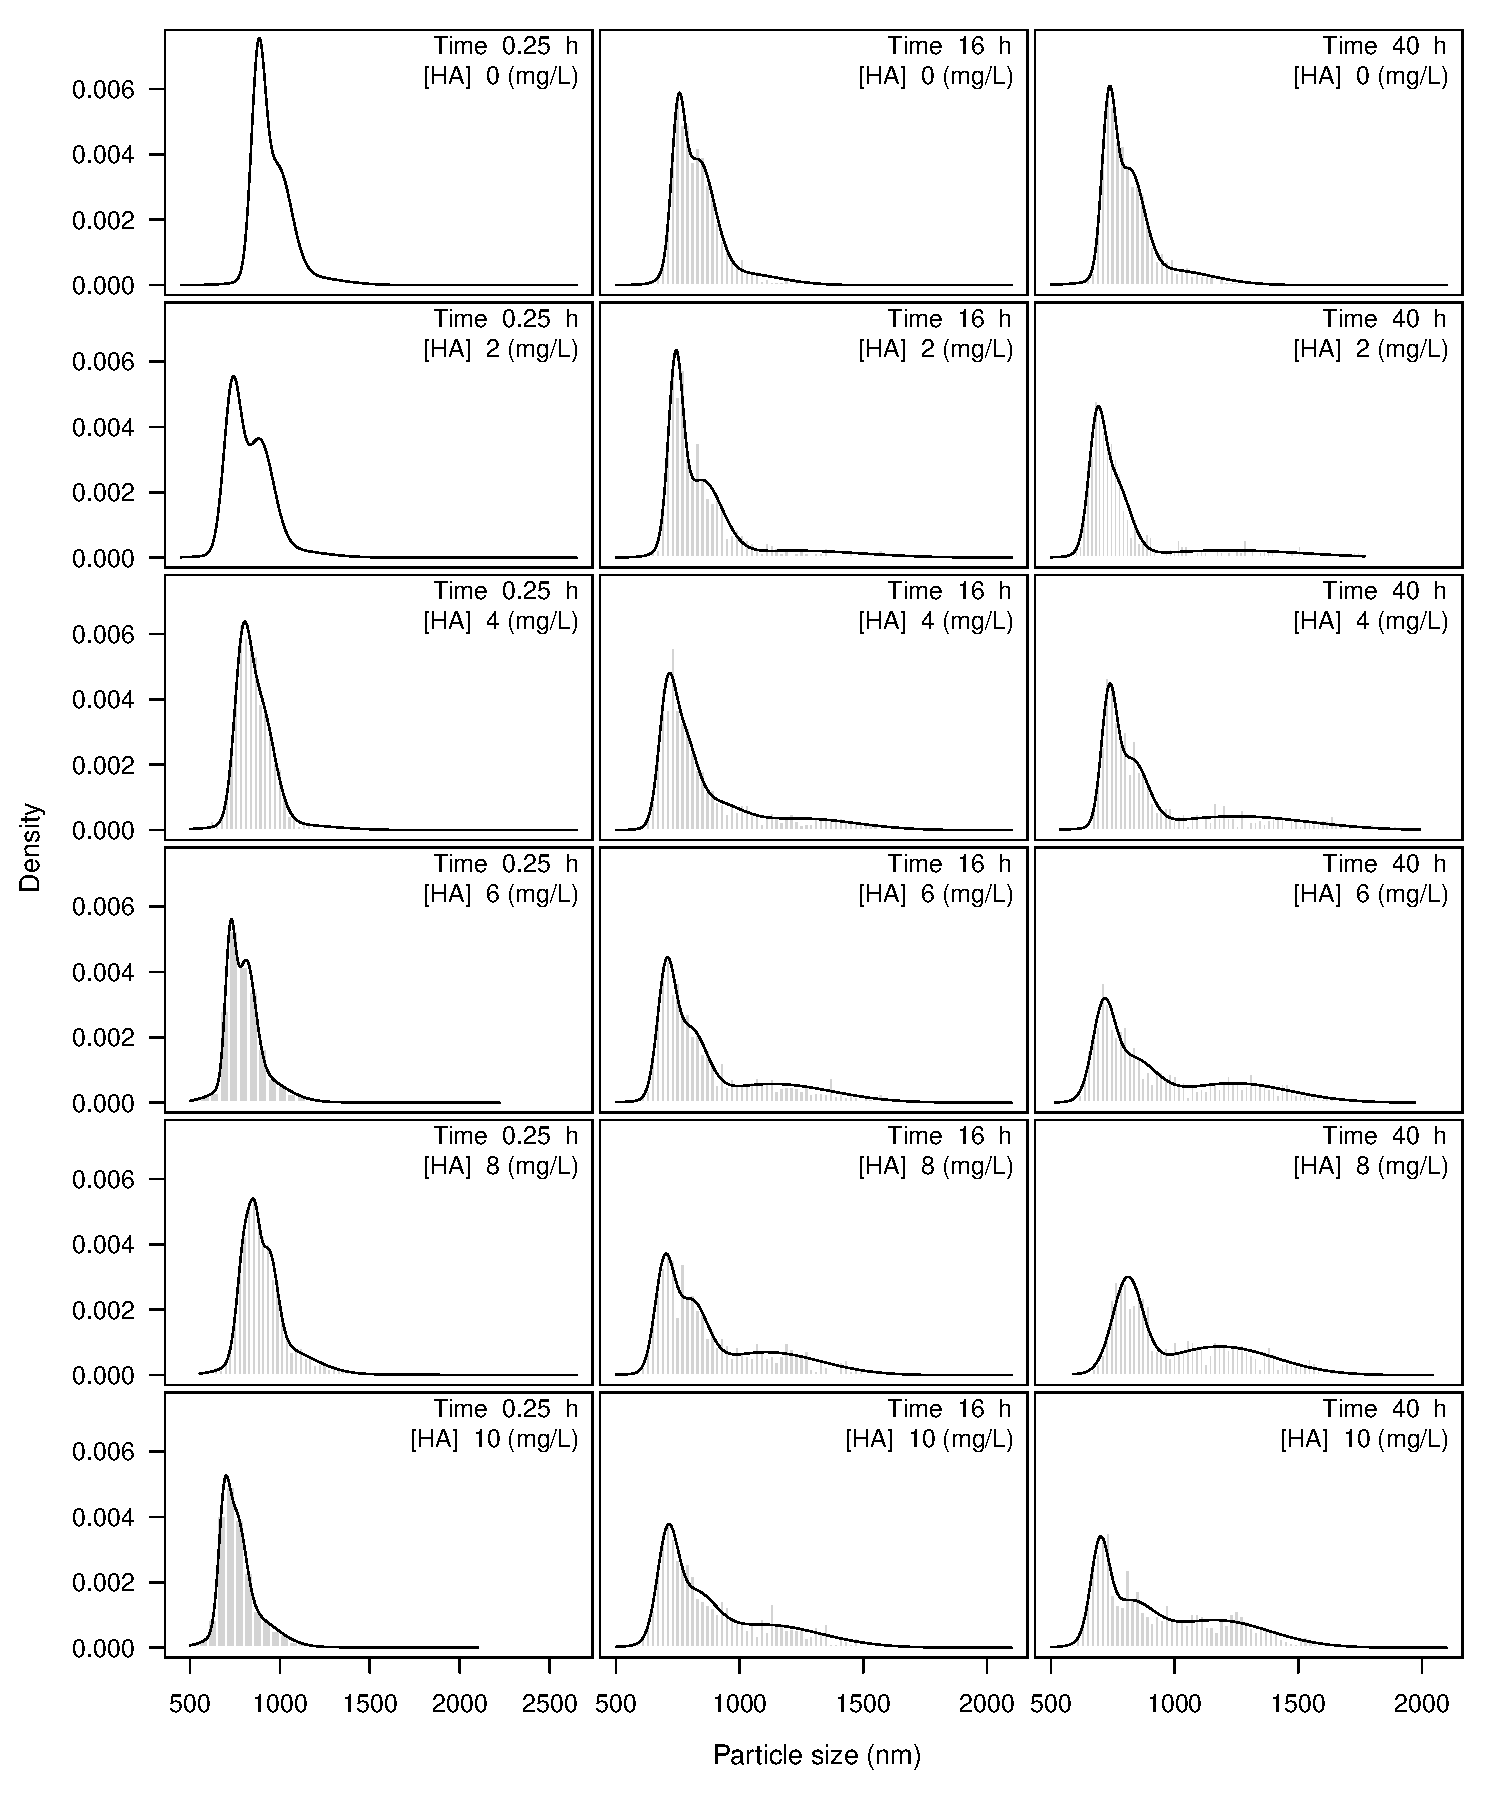
\includegraphics[width=\linewidth]{Figures/MCluster_MS_HA_density.pdf}
  \caption{Histograms and best fitting kernel density function (line) describing the influence of the incubation time and the concentration of humic acids over the particle size distribution (determined by tunable resistive pulse sensing). Plots show multiple components and density shifts towards larger sizes with the increasing of the concentration of humic acids and the incubation time. In all determinations, the number of blockades was greater than $500$.} 
  \label{fgr:multiplot_density}
\end{figure}
%%=============================================================



%%============================================================= 
 \begin{figure}
  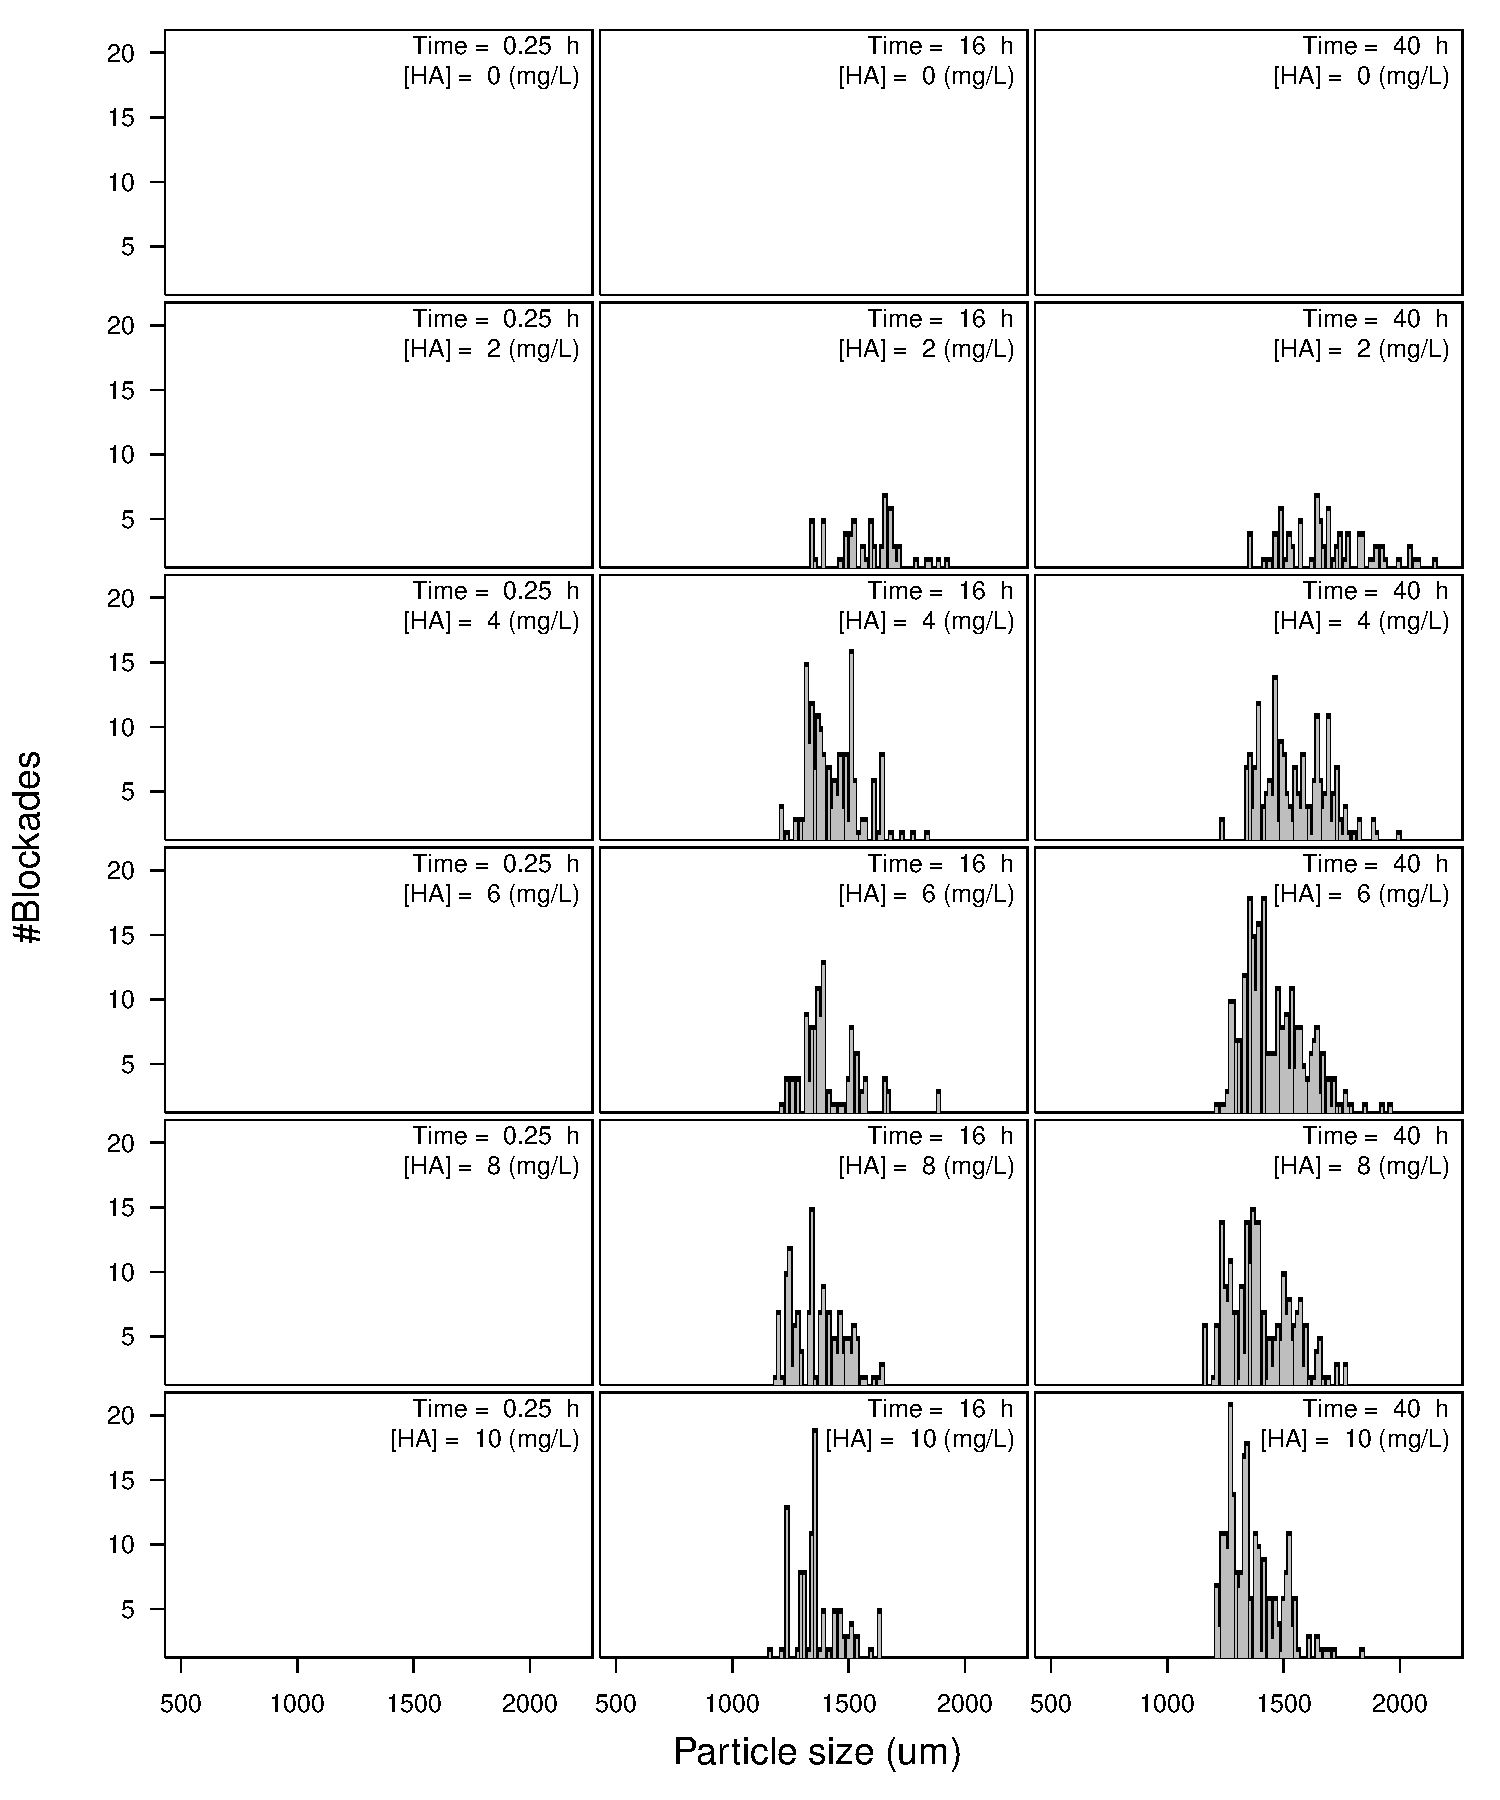
\includegraphics[width=\linewidth]{Figures/HA_density.pdf}
  \caption{Influence of the HA on the blockade counting of microspheres. \#Blockades is the difference between the number of blockades in presence of HA and the number of blockades in absence of HA at incubation times = 0.25 h.} 
  \label{fgr:HA_density}
\end{figure}
% * <diego.cerreda@gmail.com> 2017-06-19T15:20:10.367Z:
% 
% > \begin{figure}
% >   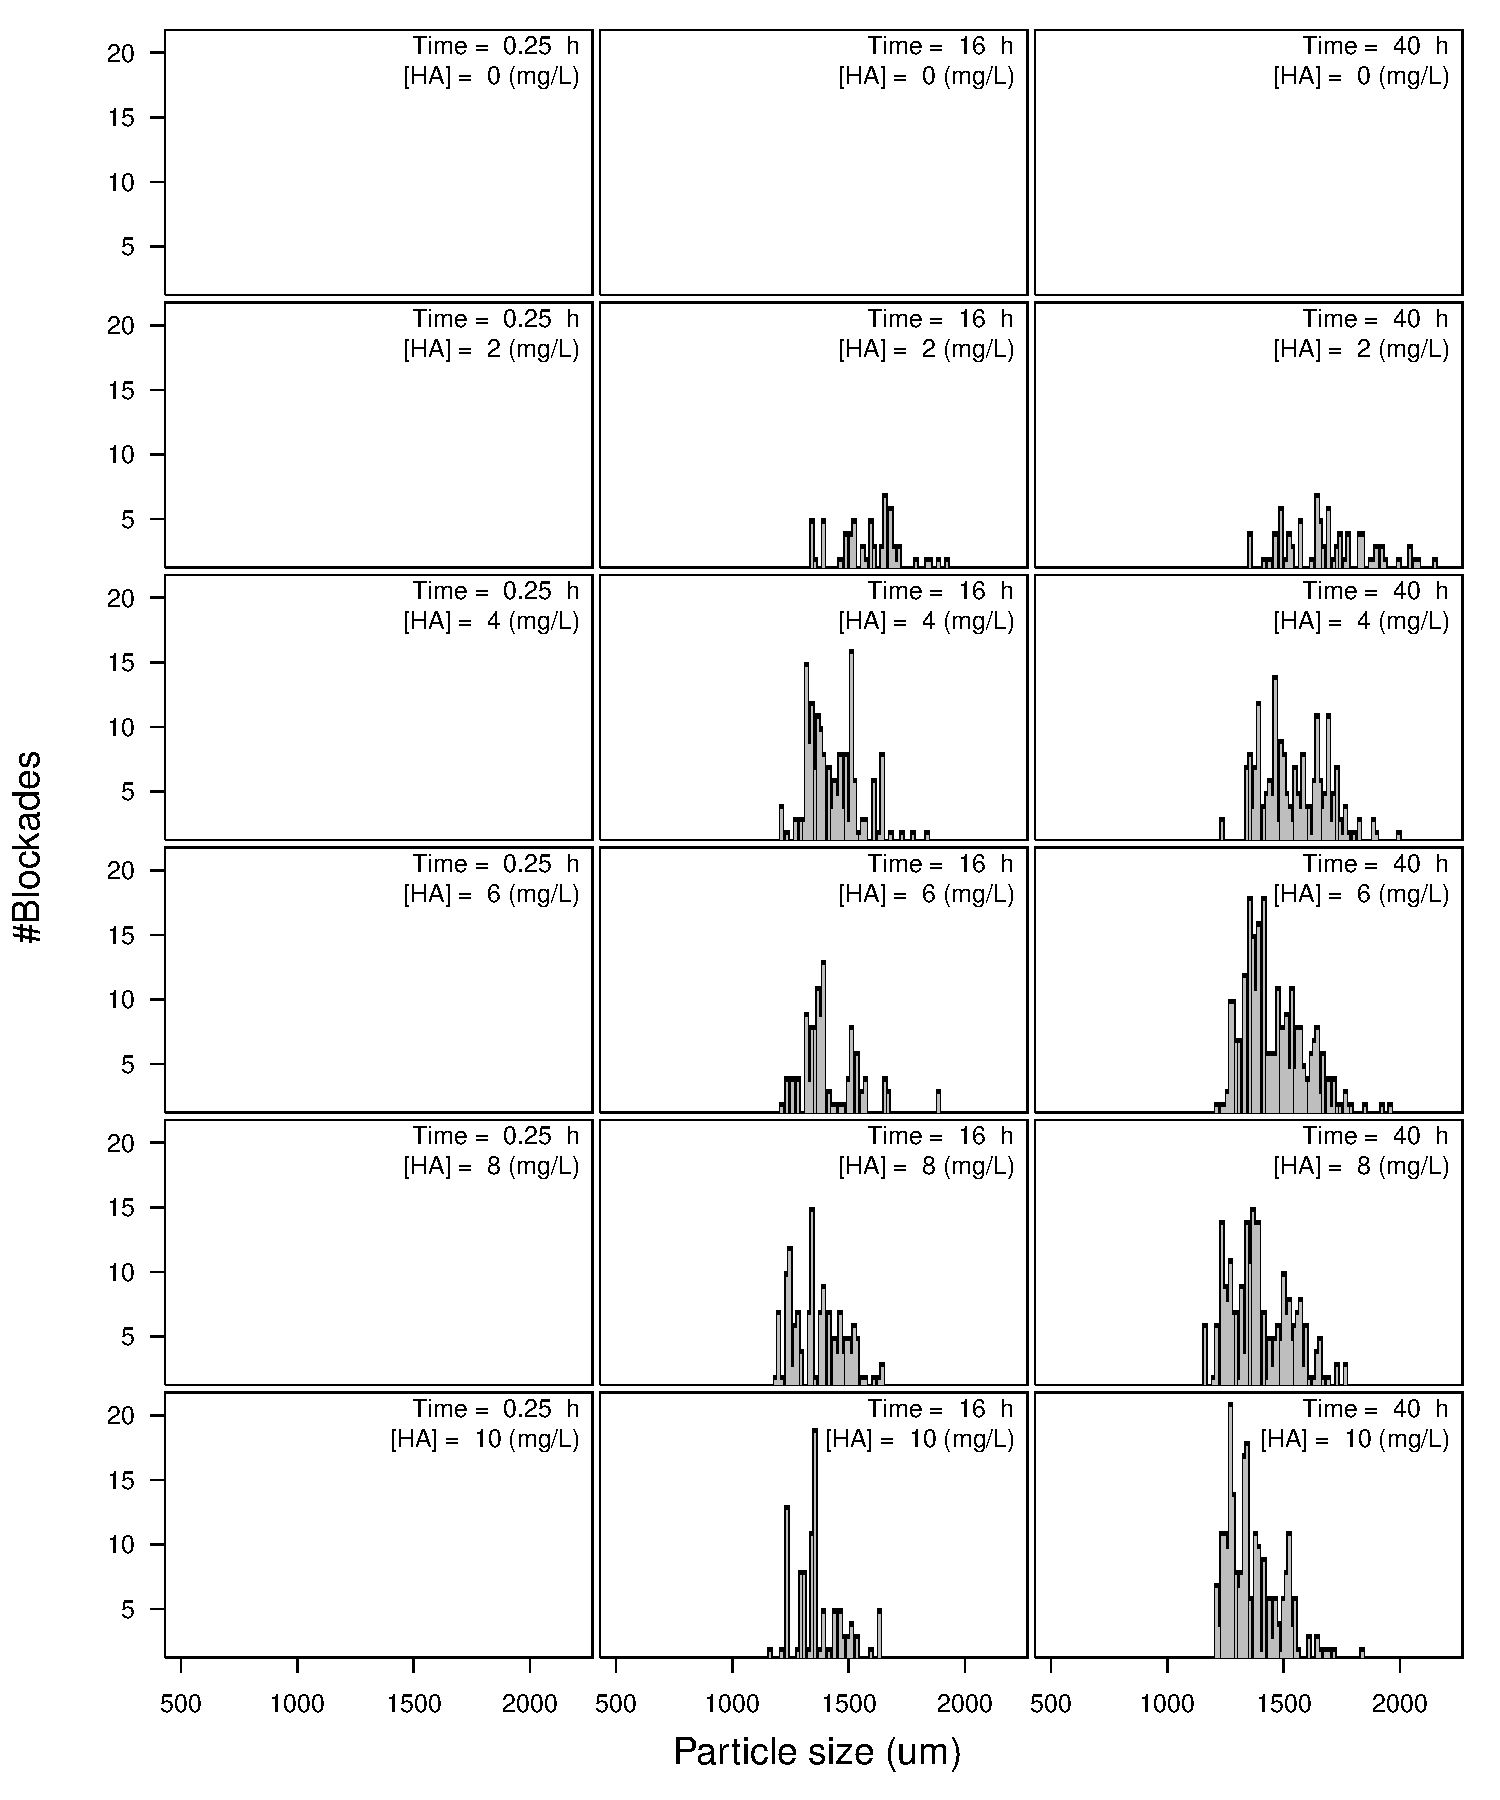
\includegraphics[width=\linewidth]{Figures/HA_density.pdf}
% >   \caption{Influence of the HA on the blockade counting of microspheres. \#Blockades is the difference between the number of blockades in presence of HA and the number of blockades in absence of HA at incubation times = 0.25 h.} 
% >   \label{fgr:HA_density}
% > \end{figure}
% 
% Nombre del eje. Particle size (nm)
% 
% ^.
%% ============================================================


\begin{table}
\label{tbl:sizes}
\caption{Mean and variance of particle diameter measured by TRPS that correspond to the best fitting gaussians obtained from the EM clustering algorithm. Values are displayed for each of the [HA] and incubation times of MS and HA in \ce{CaCl2}.}
\begin{tabular}{r r rr rr rr}
[HA] &Time &
mean  & var.  &
mean  & var.  &
mean  & var.  \\
\hline
& & \multicolumn{2}{c}{Cluster 1}&
\multicolumn{2}{c}{Cluster 2}&
\multicolumn{2}{c}{Cluster 3} \\
\hline  
 0 & 0.25 & 713 & 991 & 787 & 4543 & 866 & 31755 \\ 
 0 & 16 & 969 & 1852 & 909 & 207 & 1069 & 60279 \\ 
 0 & 40 & 731 & 855 & 813 & 3000 & 959 & 27462 \\ 
 2 & 0.25 & 709 & 1037 & 798 & 3627 & 841 & 22213 \\ 
 2 & 16 & 762 & 2053 & 882 & 11813 & 1453 & 51244 \\ 
 2 & 40 & 737 & 1712 & 838 & 8097 & 1461& 52821 \\ 
 6 & 0.25 & 711 & 1087 & 796 & 2908 & 896 & 49951 \\ 
 6 & 16 & 700 & 639 & 776 & 4396 & 1120 & 66499 \\ 
 6 & 40 & 754 & 3051 & 872 & 13321 & 1393 & 50979 \\ 
 6 & 0.25 & 698 & 1303 & 782 & 4260 & 921 & 47950 \\ 
 6 & 16 & 704 & 985 & 794 & 4215 & 1078 & 56600 \\ 
 6 & 40 & 721 & 2122 & 830 & 12745 & 1272 & 71453 \\ 
 8 & 0.25 & 695 & 632 & 779 & 4667 & 903 & 32813 \\ 
 8 & 16 & 698 & 1299 & 797 & 5097 & 1112 & 52125 \\ 
 8 & 40 & 707 & 2561 & 806 & 6201 & 1119 & 55612 \\ 
 10 & 0.25 & 703 & 1341 & 789 & 8548 & 981 & 63088 \\ 
 10 & 16 & 702 & 1336 & 810 & 3700 & 1057 & 49303 \\ 
 10 & 40 & 729 & 3537 & 982 & 17527 & 1200 & 45689 \\ 
\hline
\multicolumn{8}{l}{[HA] in $\mathrm{mg\,L^{-1}}$; Time in $\mathrm{h}$; mean and variance (var.) in $\mathrm{nm}$.} 
\end{tabular}
\end{table}


%=========================================================================

Figure~\ref{fgr:boxplot_size} shows the results of the particle size decomposition in three different clusters. Note that particle size in the cluster no.~1 is smaller than the nominal particle size provided by the supplier. 
%This is because this nominal size was used as reference size for calibration. Therefore, considering that the microspheres used in the calibration of the TRPS are fairly polydisperse, the clustering separate populations both, below and above  the nominal size.
%revisar esto
The cluster no.~2 is on the particle size reported by the manufacturer, and the cluster no.~3 is above. That indicates that TRPS detects polydispersivity of the MS standards at early times, in our case after 5 min of incubation, in presence of \ce{CaCl2} and in the absence of HA.
%% Cluster numero 1 azul 
The cluster no.~1 groups the particles in the range from $700$ to $810\;\mathrm{nm}$. The size of the particles in this cluster did remained unchanged with the incubation time and the HA concentration. That means that there is a significant population of MS whose size was not influenced by the HAs. The largest deviations in the particle size distribution (PSD) corresponded to the absence of HA and the smaller concentration, $\mathrm{[HA]  = 2\,mg\;L^{-1}}$.
%Recall that 
%$\mathrm{[HA] =\; 2\; mg\,L^{-1}}$
%was about 30~times the stoichometric rate required for  coating the MS with a monolayer of HA.
This can by caused by the separation process: the distinction between clusters at low [HA] and early times is not well defined. For example, in absence of HA at $16~\mathrm{h}$ of incubation, the populations assigned to clusters 1 and 2 are very close to each other. On the contrary, with larger HA concentrations and long  times, cluster separation is neat.


%% Cluster numero 2 verde 
The cluster no.~2 groups the particles with a size in the range from $810$ to $980\;\mathrm{nm}$. Clusters no.~1 and 2 rarely overlap, that only happens with some extreme values with [HA]$\leq\, 2\;\mathrm{mg\,L^{-1}}$. With times between $0 -16~\mathrm{h}$, and [HA] in the range of $4 - 6~\mathrm{mg\, L^{-1}}$, the variance of particle size distribution decreased, and the size regarding the smaller [HA]. Large variances  and sizes at low [HA] and times $< 16~\mathrm{h}$ are a ''statistical artifact'' that results from the unclear separation of the particle size components. So that, this does not represent a true population. There is an increase of the particle size in the interval of [HA] $4-10~\mathrm{mg\,L^{-1}}$. This rate of increase in diameter was $4.6\,\pm 1.8~\mathrm{nm\,L\,mg^{-1}}$, with a $\mathrm{P = 0.027}$ $r^2 > 0.635$ and 11 degrees of freedom. 
% * <diego.cerreda@gmail.com> 2017-06-19T16:03:42.359Z:
% 
% >  $\mathrm{P = 0.027}$ $r^2 > 0.635$ 
% Esto está ben¿?
% 
% ^.
That confirms that the size of particles in the cluster no. 2 increases significantly with the [HA], and the growth rate manifests at $16~\mathrm{h}$ incubation.

% Pendiente de Realizar puebas estadisticas del modelo lineal (tamaño ~[HA])


%%Cluster numero 3 rojo.
Cluster no. 3 groups the particles with the largest size ($> 980~\mathrm{nm}$).  At short times, $0.25~\mathrm{h}$, there was a monotonic increase in size with the [HA] in the range $2-8~\mathrm{mg\,L^{-1}}$. At larger contact times, $16-40~\mathrm{h}$, the size increased dramatically with a maximum at $\mathrm{[HA]} = 2~\mathrm{mg\,L^{-1}}$. Then, at higher [HA] the size  diminished with an uniform decrease that can be clearly observed at 
$40~\mathrm{h}$. The highest size, $1462~\mathrm{nm}$, was measured with $\mathrm{[HA]} = 2~\mathrm{mg\,L^{-1}}
$ at  $40~\mathrm{h}$. This maximum is twice the size of the particles of the cluster no. 1, indicating that this size may correspond to MS aggregates. 
%Laura: comprobar con microscopía, tenemos fotos?

%%========================================================================= 
 \begin{figure}
  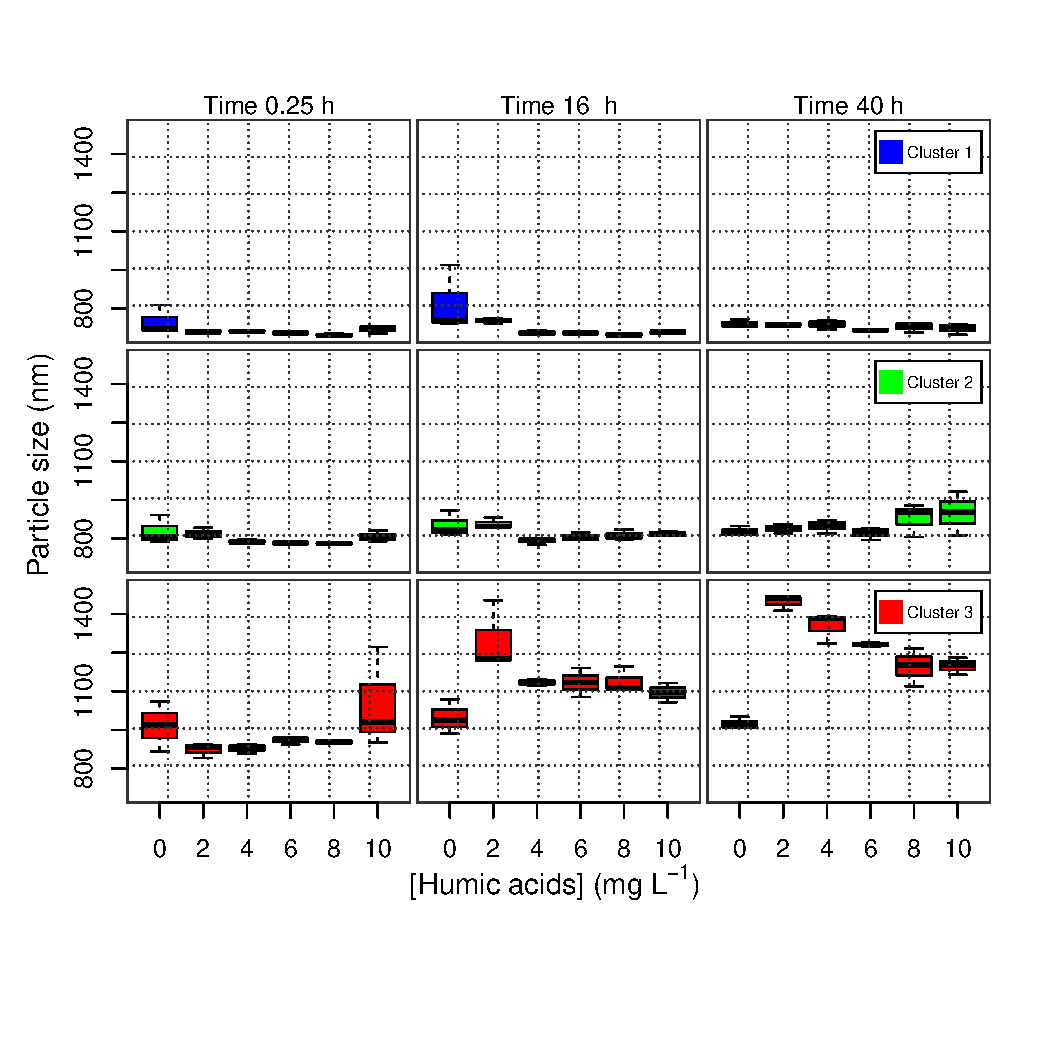
\includegraphics[width=\linewidth]{Figures/Boxplot_MS_HA_CaCl2_sizes.pdf}
  \caption{Influence of the concentration of Humic Acids and contact time on the  size of microspheres.  Clusters numbered from 1 to 3 correspond to three gaussians that were identified by optimal fitting using the expectation maximization (EM) algorithm  that minimizes the Bayesian Information Criterion (BIC). The incubation times of the MS,  namely 0.25, 16 and 40, are indicated by labels on the top of the panels.}
  \label{fgr:boxplot_size}
\end{figure}
%%======================================================================== 





%%=========================================================================
\subsection{Distribution of particle populations}
% En esta parte solamente describimos los resultados, no aventuramos ninguna 
% hipótesis porque no sabemos que es lo que ocurre realmente.
% Puede ocurrir que e  el cluster 1 solamente existan MS, y en los demás
% clusters solamente existan HA floculados.
% Así que estamos a la espera de los resultados de Laura.

Classification of particles in different apparent sizes was used to analyze the changes in the population distribution in function of time and [HA]. Figure~\ref{fgr:boxplot_populations} shows the distribution of populations, namely, the frequency of particle counts in each size fraction regarding the influence of [HA].

%Analisis de las poblaciones en el Cluster 1 azul
Populations in the cluster no .1 constitute less than the half of the TRPS counts. This cluster do not show a clear relation with the [HA] or with the time. Only  shows a  significant decrease with the [HA in the range $2-6~\mathrm{mg\,L^{-1}}$ at $40~\mathrm{h}$ that can be related to the increase of the larger particles in the cluster no. 3 in the same conditions of [HA] and incubation time.

%Analisis de las poblaciones en el Cluster 2 verde
Cluster no. 2 encompassed the higher number of counts, i.e. $>\,0.5$ population fraction, at short times ,$0.25~\mathrm{h}$, with a significant decrease at bigger [HA], $>8~\mathrm{mg\,L^{-1}}$. At larger times, the population decreased significantly in the range of [HA] $2-8~\mathrm{mg\,L^{-1}}$. Changes in the particle populations in the cluster no. 2 do not have significant correspondence  with the variations in the cluster no. 1. However, we can observe the same trend with [HA] $2-6~\mathrm{mg\,L^{-1}}$at $40~\mathrm{h}$.

%Analisis de las poblaciones en el Cluster 3 rojo
In Cluster no. 3 populations varied in a opposite way as in the no. 2. Figure~\ref{fgr:boxplot_populations} shows a clear increase in the population fraction with the [HA] and the contact time. This increase corresponds to a decrease in the particle counts in the cluster no. 2, and regarding [HA] is not strictly monotonic. At $\mathrm{[HA]} = 2~\mathrm{mg\,L^{-1}}$, the  population reached the  minimum: $0.12$  and $0.15$. These apparent sizes correspond with the largest sizes, $1300~\mathrm{nm}$ at $16~\mathrm{h}$ and $1462~\mathrm{nm}$ at $40~\mathrm{h}$, doubling the diameter of the primary MS. That decrease mimics the flocculation behavior at $\mathrm{[HA]} = 2~\mathrm{mg\,L^{-1}}$discussed above. ,



%===========================================================================
\begin{figure}
 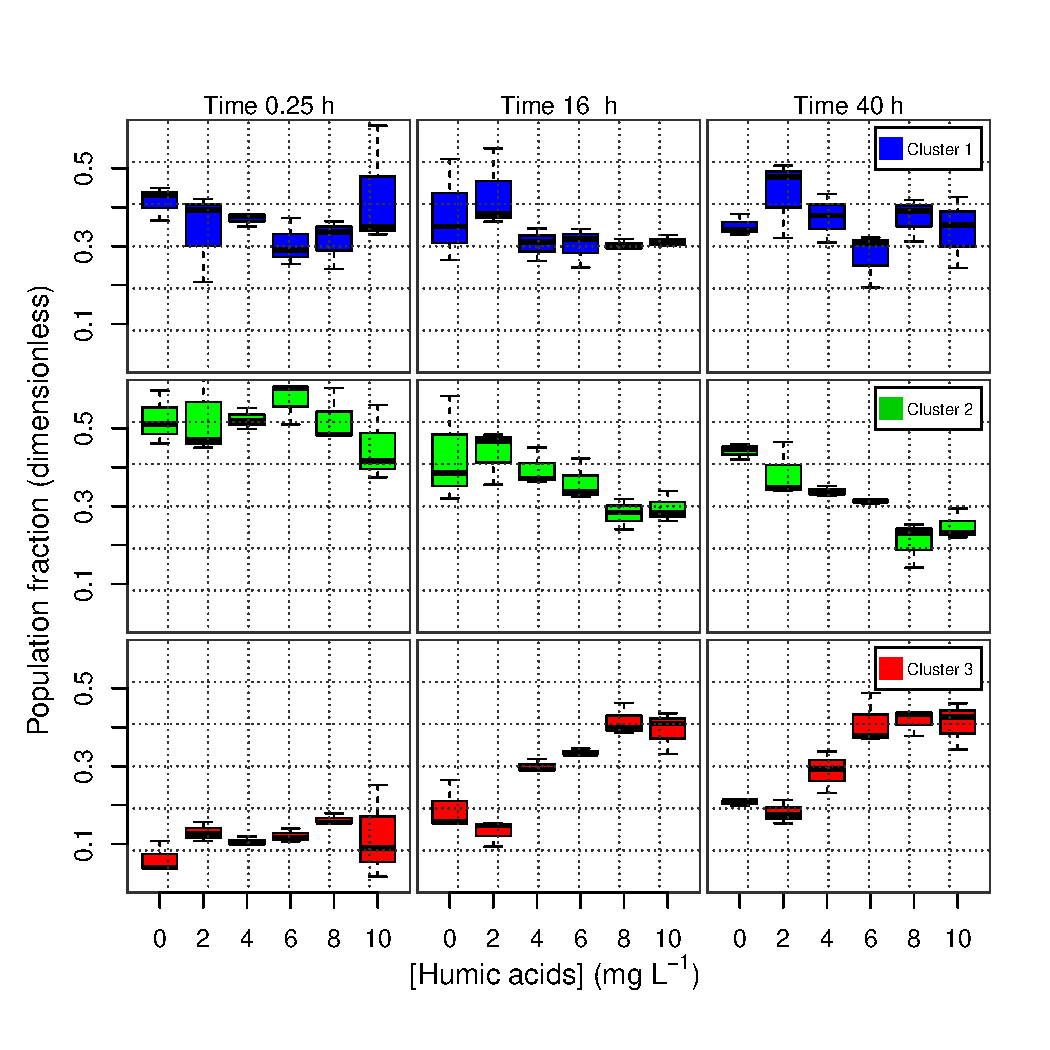
\includegraphics[width=\linewidth]{Figures/Boxplot_MS_HA_CaCl2_populations.pdf}
  \caption{Influence of the Humic Acids concentration and contact time on the population distribution of MS into three particle size fractions denoted as
  Cluster 1 ($700 - 810~\mathrm{nm}$),  Cluster 2 ($810 - 980~\mathrm{nm}$), 
  and
  Cluster 3 ($ > 980~\mathrm{nm}$)
  }
  \label{fgr:boxplot_populations}
\end{figure}
%===========================================================================





%%=====================================================================
%%Discussion
%%=====================================================================

\section{Discussion}


%
The suitability of TRPS to study colloid particle sizes is limited by the current intensity that crosses the measuring pore, and  that depends on the electrolyte composition. Fortunately, the optimal pH and \ce{[Ca^{2+}]} for the TRPS measurements falls into the typical values of the soil solution\cite{wolt1994soil} and  fresh water environments\cite{Stumm1993}. Therefore, TRPS can be used to characterize colloidal suspensions in many  aquatic samples and soil water extracts.

%HA-MS interaction
Theoretical calculations and SEM images showed that adsorption of  HA on latex microspheres is negligible. The HA-MS mixture is a charged-neutral system, so the charge regulation effects depend on the adsorption of ions to the surface. The regulation parameter for the neutral latex microspheres, $P$, can vary between -1 (attractive) net energy interaction and 1  (repulsive). In the constant charge boundary conditions predict  repulsive forces at few nm separation distance, while constant potential condition predicts and attractive force\cite{Trefalt2014}. A constant regulation condition can be roughly estimated from the  colloidal probe technique based on the atomic force microscope\cite{Ruiz-Cabello2013}.
For weak attractive potentials, the diffuse layer thickness is much larger than the potential distance. The conformation of a large  polymer weakly adsorbed is similar to the unperturbed one far from the surface\cite{Netz2003}. Therefore, conformation changes of HA induced by their proximity to the MS can not be expected.

%Discusión: floculacion excesiva por elevada fuerza iónica
Large aggregates exceeding  the size of the measurement pore in the TRPS cannot be measured with precision. An alternative is using a  large pore, however large pores penalize accuracy of particles so small that are below the pore measurement range.


%quedei
%Dicussion: Que pasa con los dos clusterings del MS-calcio sin HA?
The blockade duration is related to the passing time across the pore membrane. So that longer blockade durations can be assigned to differences in the surface potential.
\citeauthor{Weatherall2016}
\citeyear{Weatherall2016}.
% Aqui discutimos la parte de la \subsection{Clustering particle sizes}

From this observation  some findings about the HA-MS interactions in presence of \ce{Ca^{2+}} can be drawn.
%First consider that the reference standards MS is not a single unimodal population.
%Laura: pedirle los  datos de las cuentas de calibración para comprobar mediante clustering si la distribución es unimodal o no
%TRPS and clustering confirm the reported using flow cytometry, that the population can be optimally described by three gaussians.
 First, the  high resolution DLS procedure suggested by
 ~\citeauthor{Bryant2003AccurateSuspensions}\cite{Bryant2003AccurateSuspensions} 
reported  that poly(methyl methacrylate)-based particles have negatively
skewed particle size distributions, and in many cases could be characterized
by the Weibull extreme value distribution. This type of distribution 
was also found by fitting the overall particle size distribution obtained by TRPS. However, statistical clustering of TRPS data can resolve different components.


% Comparar métodos con los resultados que tenemos con citometria de flujo: Buscar las figuras de citometría de los resultados de Almudena.
%%
Second, Cluster no. 1 encompasses a fraction of MS (Figure~\ref{fgr:boxplot_populations}) that is not influenced by the presence of HA, even in presence of \ce{CaCl2} and HA at concentrations several times higher than the level needed for the complete covering of the MS surface.
%%


Third, the behavior of the the intermediate component (cluster no. 2) clearly indicates an increase in the particle size associated with the [HA] and
contact time. The coexistence of different sizes and the
slow  growth rate indicate that the kinetics of HA binding
to MS is slow. Adsorption of HA on MS is limited by
transport and electrostatic interactions~ \cite{doi:10.1021/es981236u}.
Double layer interaction calculations (Table~\ref{tbl:dvlo_interaction}) showed a low  repulsion barrier,
so that the attraction force is small and the range of electrostatic attraction is short $\sim 20~\mathrm{nm}$.
The rate of increase in size is about one  layer of primary particles of HA per $\mathrm{mg HA\,L^{-1}}$ in the suspension.

%%
Fourth, the dramatic increase in size in cluster no. 3 
and subsequent decrease indicates bridging flocculation at 
$\mathrm{[HA] \,=\, 2\;mg\,L^{-1}}$, followed by polymer stabilization at higher [HA]. %% Pendiente de confirmar por microscopía.
Bridging flocculation and polymer stabilization can occur, in presence of \ce{Ca^{2+}}, to any colloid that adsorbs dissolved organic matter and .

Transition from bridging flocculation to polymer stabilization results from the stoichometry ratio of 
\ce{Ca^{2+}}:HA.
With 
$\mathrm{[HA]} = 2~\mathrm{mg\,L^{-1}}$ there is enough 
\ce{Ca^{2+}} to stabilize HA-MS bindings. However, at higher concentrations
the most
\ce{Ca^{2+}}
can be  complexed by the excess of HA  so that little
\ce{Ca^{2+}}
is available to strength the polymer bridges between ms.
The overall mechanism  result in a slow thickening of the MS coating. 

%=================================================
\section{Conclusions}


TRPS provides a very good resolution in the separation  of particle sizes in polydisperse mixtures, better than alternative techniques to study surface adsorption, such as laser-beam reflectometry. However, that separation must be accompanied by a careful statistical clustering procedure. The quality of separation depends on the neatness definition of subpopulations. A continuous broad distribution of particle sizes cannot bring a statistical separation.
The presence of HA in the micropore increases the blockade magnitude of the passing microspheres, causing an overestimation of the size measured by TRPS.  The linear relationship  between particle size growth and [HA] sketches new potential methods based on TRPS to quantify the influence of the coating of MS by HA on the particle thickening.

%=========================================================================
Results  point the role of dissolved organic polymers on the behavior of colloidal particles in soils and porous media in general. So, can contribute in fields related to 
water quality, environment, and public health.
%=========================================================================



%%%%%%%%%%%%%%%%%%%%%%%%%%%%%%%%%%%%%%%%%%%%%%%%%%%%%%%%%%%%%%%%%%%%%
%% The "Acknowledgement" section can be given in all manuscript
%% classes.  This should be given within the "acknowledgement"
%% environment, which will make the correct section or running title.
%%%%%%%%%%%%%%%%%%%%%%%%%%%%%%%%%%%%%%%%%%%%%%%%%%%%%%%%%%%%%%%%%%%%%
\begin{acknowledgement}

%The authors thanks 
%Camille Roesch, Izon Europe Ltd. for technical supporting the TRPS.
This
work is partially funded by an AA1-GRC research contract (UE-FEDER,
Xunta de Galicia GRC2014/017), Diego-Soto by Spanish Government MEC’s FPU.

\end{acknowledgement}

%%%%%%%%%%%%%%%%%%%%%%%%%%%%%%%%%%%%%%%%%%%%%%%%%%%%%%%%%%%%%%%%%%%%%
% The same is true for Supporting Information, which should use the
%% suppinfo environment.
%%%%%%%%%%%%%%%%%%%%%%%%%%%%%%%%%%%%%%%%%%%%%%%%%%%%%%%%%%%%%%%%%%%%%
\begin{suppinfo}

This will usually read something like: ``Experimental procedures and
characterization data for all new compounds. The class will
automatically add a sentence pointing to the information on-line:

\end{suppinfo}

%%%%%%%%%%%%%%%%%%%%%%%%%%%%%%%%%%%%%%%%%%%%%%%%%%%%%%%%%%%%%%%%%%%%%
%% The appropriate \bibliography command should be placed here.
%% Notice that the class file automatically sets \bibliographystyle
%% and also names the section correctly.
%%%%%%%%%%%%%%%%%%%%%%%%%%%%%%%%%%%%%%%%%%%%%%%%%%%%%%%%%%%%%%%%%%%%%
\bibliography{Mendeley,Laura}

\end{document}


%% MANUAL DE USO


%New float types are automatically set up by the class file.  The
%means graphics are included as follows (Scheme~\ref{sch:example}).  As
%illustrated, the float is ``here'' if possible.
%\begin{scheme}
%  Your scheme graphic would go here: \texttt{.eps} format\\
%  for \LaTeX\, or \texttt{.pdf} (or \texttt{.png}) for pdf\LaTeX\\
%  \textsc{ChemDraw} files are best saved as \texttt{.eps} files:\\
%  these can be scaled without loss of quality, and can be\\
%  converted to \texttt{.pdf} files easily using \texttt{eps2pdf}.\\
%  %\includegraphics{graphic}
%  \caption{An example scheme}
%  \label{sch:example}
%\end{scheme}

%Adding notes to tables can be complicated.  Perhaps the easiest
%method is to generate these using the basic
%\texttt{\textbackslash textsuperscript} and
%\texttt{\textbackslash emph} macros, as illustrated %(Table~\ref{tbl:notes}).
%\begin{table}
%  \caption{A table with notes}
%  \label{tbl:notes}
%  \begin{tabular}{ll}
%    \hline
%    Header one                            & Header two \\
%    \hline
%    Entry one\textsuperscript{\emph{a}}   & Entry two  \\
%    Entry three\textsuperscript{\emph{b}} & Entry four \\
%    \hline
%  \end{tabular}
 % \textsuperscript{\emph{a}} Some text;
 % \textsuperscript{\emph{b}} Some more text.
%\end{table}